\chapter{Simple $O(n^3)$ implementation}
In this section we describe an $O(n^3)$ implementation which solves the
"Shortest Paths in Plane with Obstacles Violations"-problem. Recall that $n$ is
the number of vertices in the polygons and $k$ is the number of polygon
violations allowed. In the first section we describe how we construct the
visibility graph. Imagine a plane with a starting point $s$, an end point $t$,
and $\mathcal{O}$ polygon obstacles, which is build of groups of connected points,
each representing an obstacle. A visibility graph is a graph where for each set of
points $p,q\in \mathcal{O} \cup \{s,t\}$  there is an edge between them if the 
two points can see each other
without going (or looking) through any interior of an obstacle (see figure
\ref{visibilitygraph}). In the second section we explain Dijkstra's algorithm
for finding the shortest path from $s$ to $t$ in the visibility graph and
finally in the third section we test our implementation to compare if the actual 
running time is the same as the theoretical.

\begin{figure}[H]
	\begin{subfigure}{.5\textwidth}
		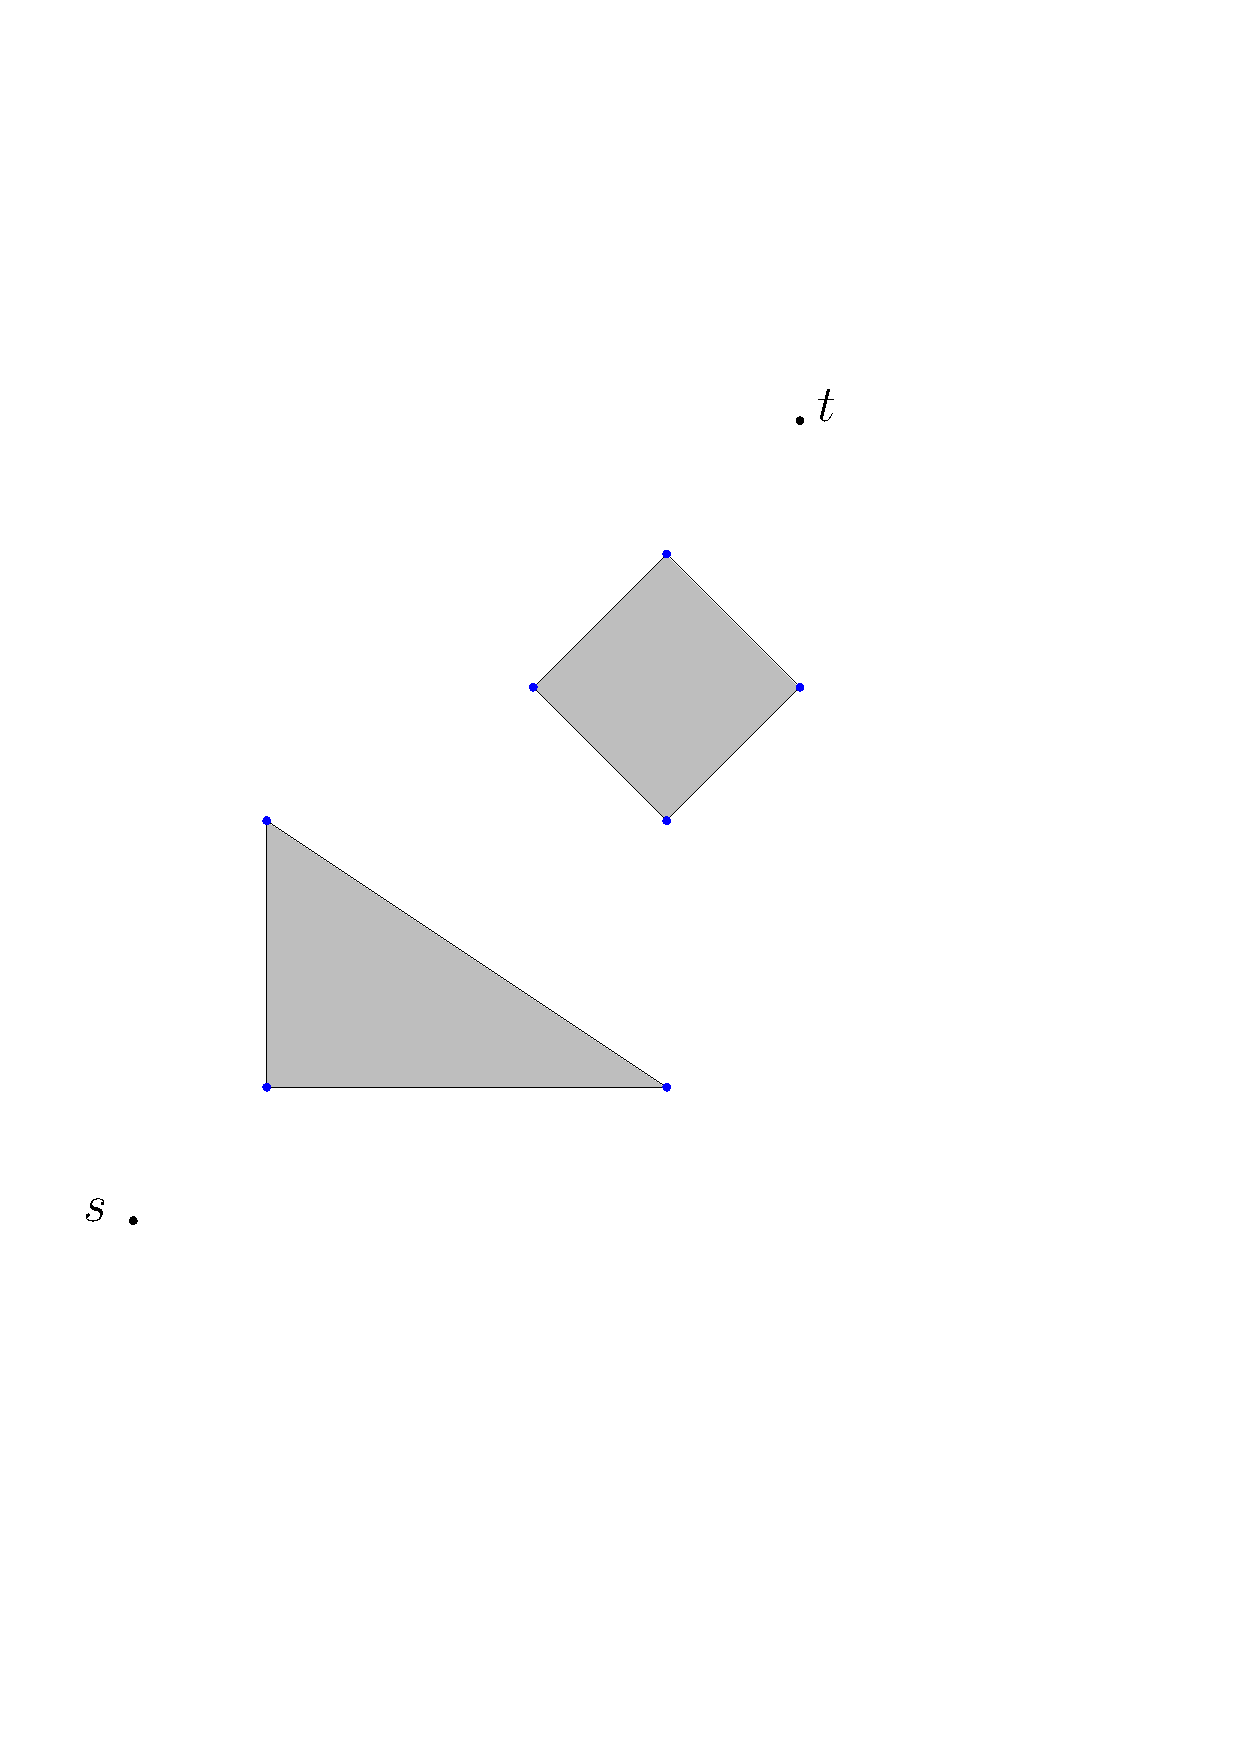
\includegraphics[width=6cm]{figures/visibilitygraph1.pdf}
		\caption{}
	\label{fig:visibilitygraph1}
	\end{subfigure}
	\begin{subfigure}{.5\textwidth}
		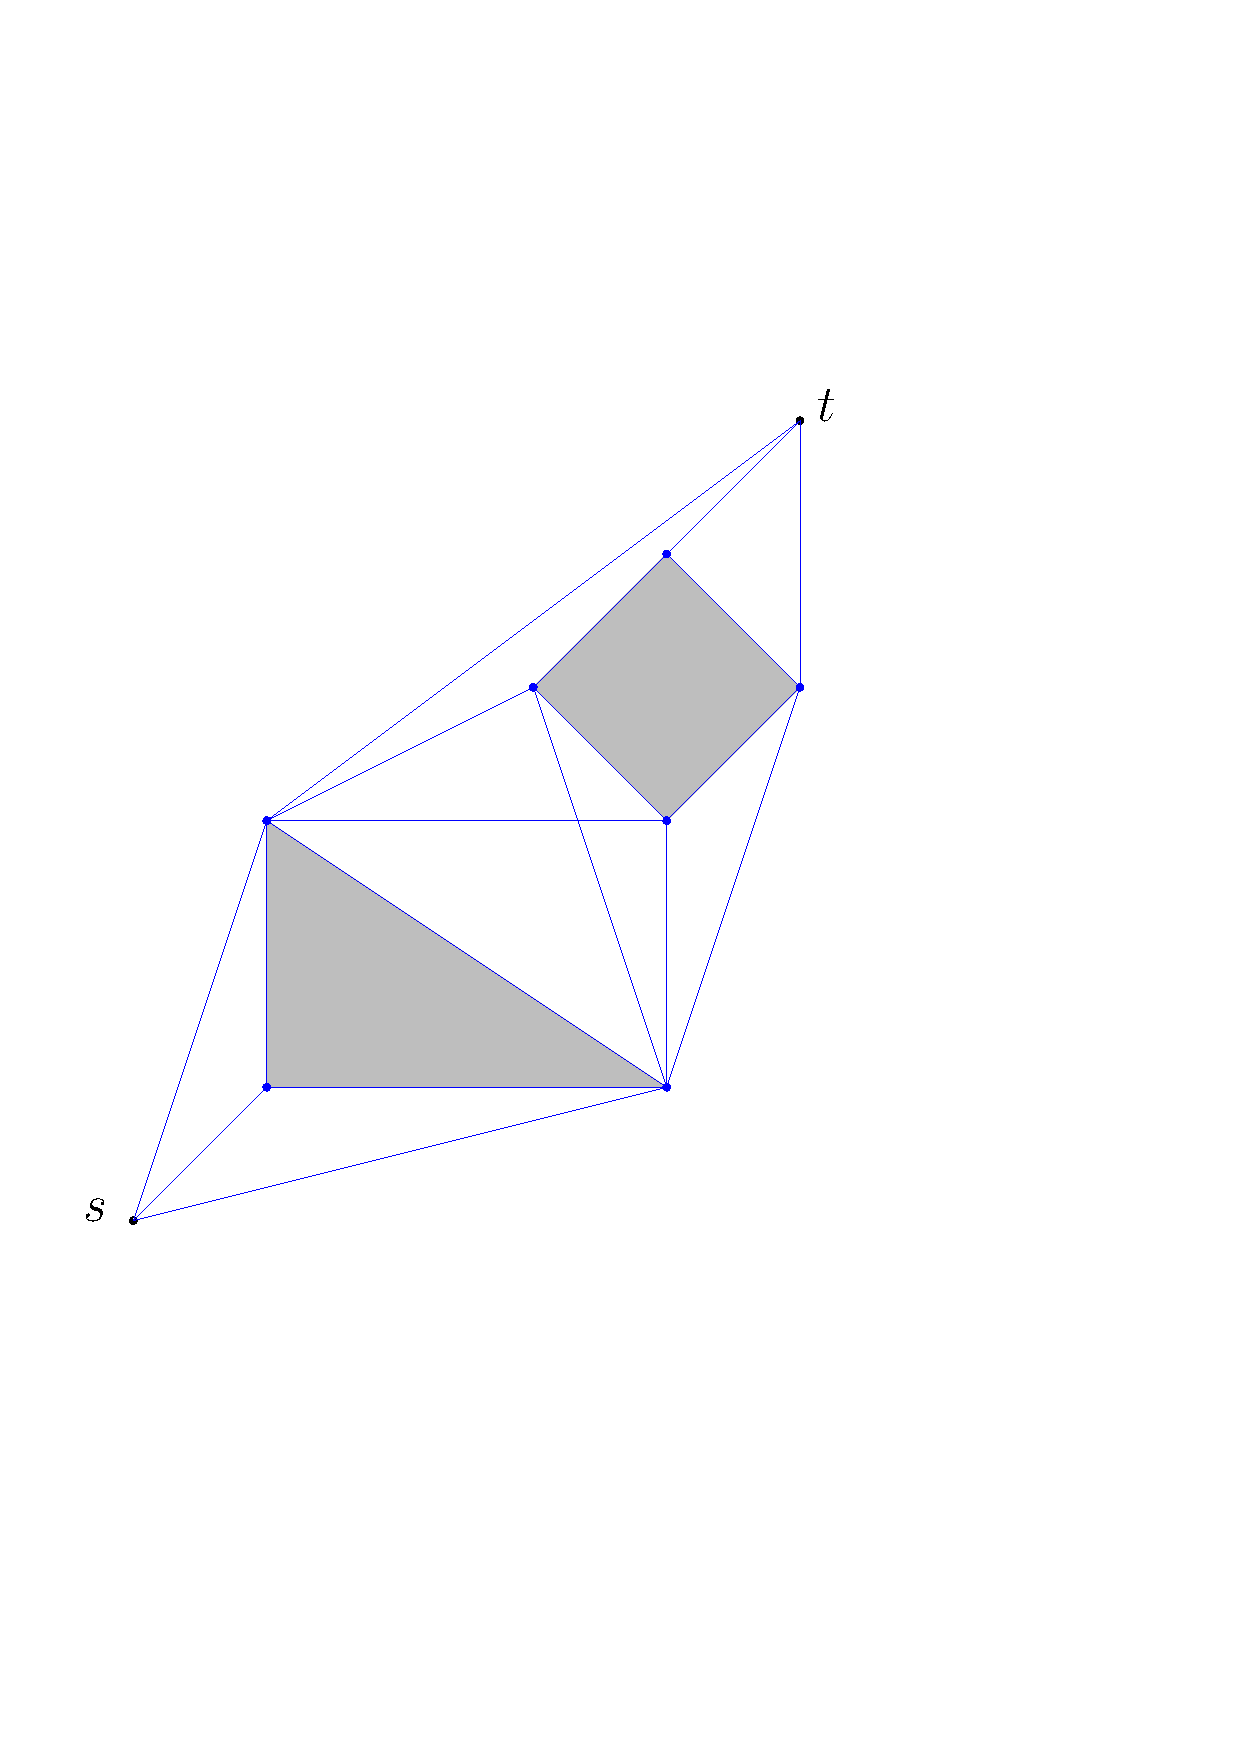
\includegraphics[width=6cm]{figures/visibilitygraph.pdf}
		\caption{}
		\label{fig:visibilitygraph2}
	\end{subfigure}
	\caption{Example of visibility graph}
	\label{visibilitygraph}
\end{figure}

\section{Constructing the visibility graph}
The naive way of constructing a visibility graph is to make a graph
where every set of points $p,q \in \mathcal{O} \cup \{s,t\}$ is connected to each other,
then removing all edges that crosses the interior of a polygon. But in this
setting we are allowed to cross $k$ polygons, so we construct the graph a bit
different. Given a set $\mathcal{O}$ consisting of all the polygons, where each polygon
is a list of the points in the polygon we use the following algorithm \ref{algo:MakeVisibilityGraph}.  
Create a graph $G_0=(V,E)$, where $V$ contains all the vertices in $P\cup \{s,t\}$,
and let $E$ contain all possible connections between the vertices. Make $k$
copies of the graph and name them $G_1,\dots,G_{k}$. Algorithm \ref{algo:MakeVisibilityGraph} goes as
follows: for each graph $G_i$, take each edge $e_j\in G_i$ and call
NumberOfCrosses$(e_j)$, which returns the number of polygons from $\mathcal{O}$ that the
line segment crosses, and connect the endpoint to the corresponding point in
$G_{i+m}$, i.e.\ if you take an edge in the graph, that goes through $m$
polygons, you travel $m$ graphs up. If $i+m > k$ then delete the edge. We now
have a graph that has $k$ levels where every time you go through $k$ polygons
you go $k$ levels up.

\begin{algorithm} 
	\caption{MakeVisibilityGraph($P,s,t$)}
	\begin{algorithmic}[1]
		\ForAll{$G_i=(V_i,E_i) \in G$}
		\ForAll{$e \in E_i$}
			\State $crosses = numberOfCrossings(e)$
			\If{$crosses+i<=k$}
				\State make $e$ go from $G_i$ to $G_{i+crosses}$
			\Else
				\State delete edge $e$
			\EndIf
		\EndFor
		\EndFor
	\end{algorithmic}
	\label{algo:MakeVisibilityGraph}
\end{algorithm}

The only missing part is the numberOfCrossings function, which we will define
below.

\subsection{Number of crossings}
Calculating the number of polygons a line segment crosses is no trivial task,
since there is a number of edge cases. We try to give a brief intuition of the
edge cases, and then present our algorithm.
The first five cases (a-e) in figure \ref{fig:crossings} are allowed intersections since
it is only the interior of a polygon that we can not travel. The
next five cases (f-j) are not allowed since they travel through the interior
of the polygon.

\begin{figure}
\begin{tabular}{|c|c|c|c|c|}
      \hline
		\multicolumn{5}{|c|}{No intersection} \\
		\hline
      \addheight{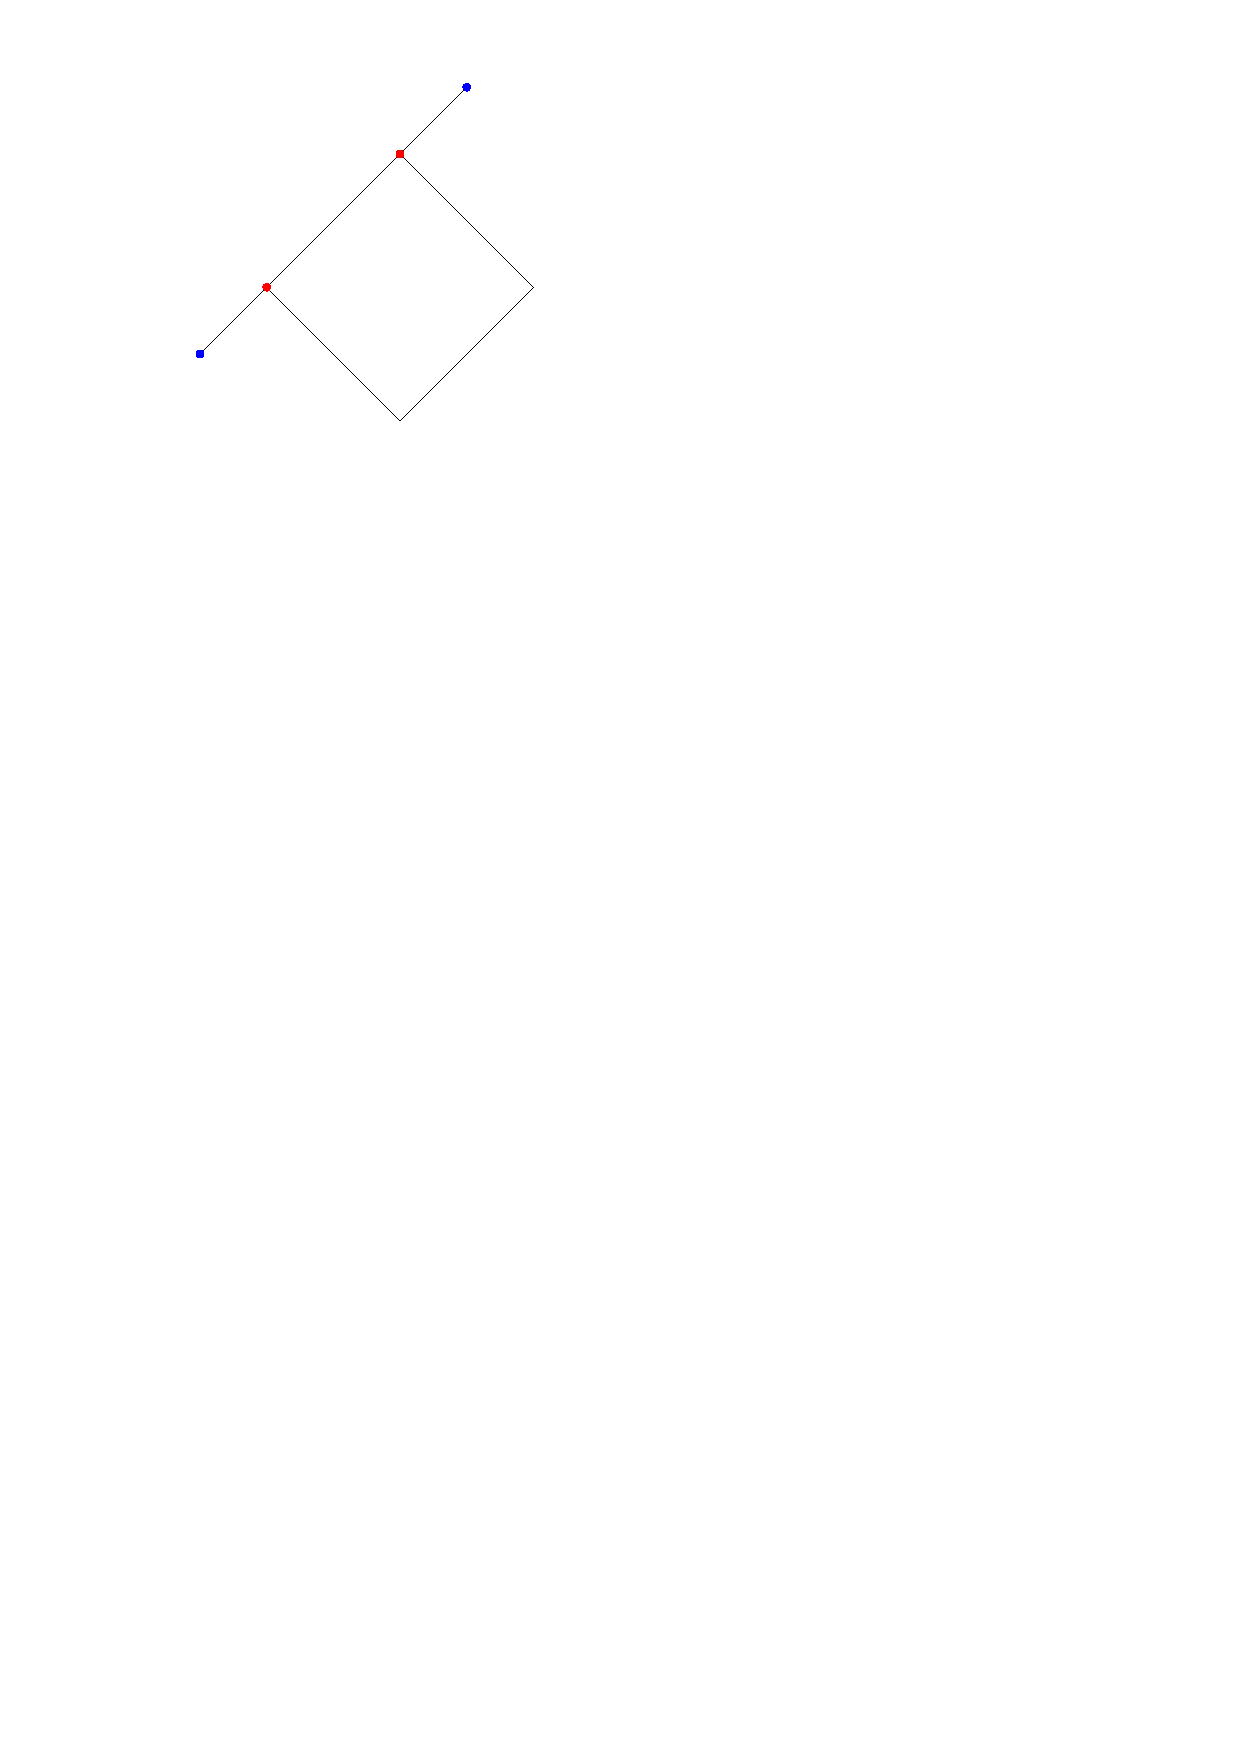
\includegraphics[width=20mm]{figures/crossFig1.pdf}} &
      \addheight{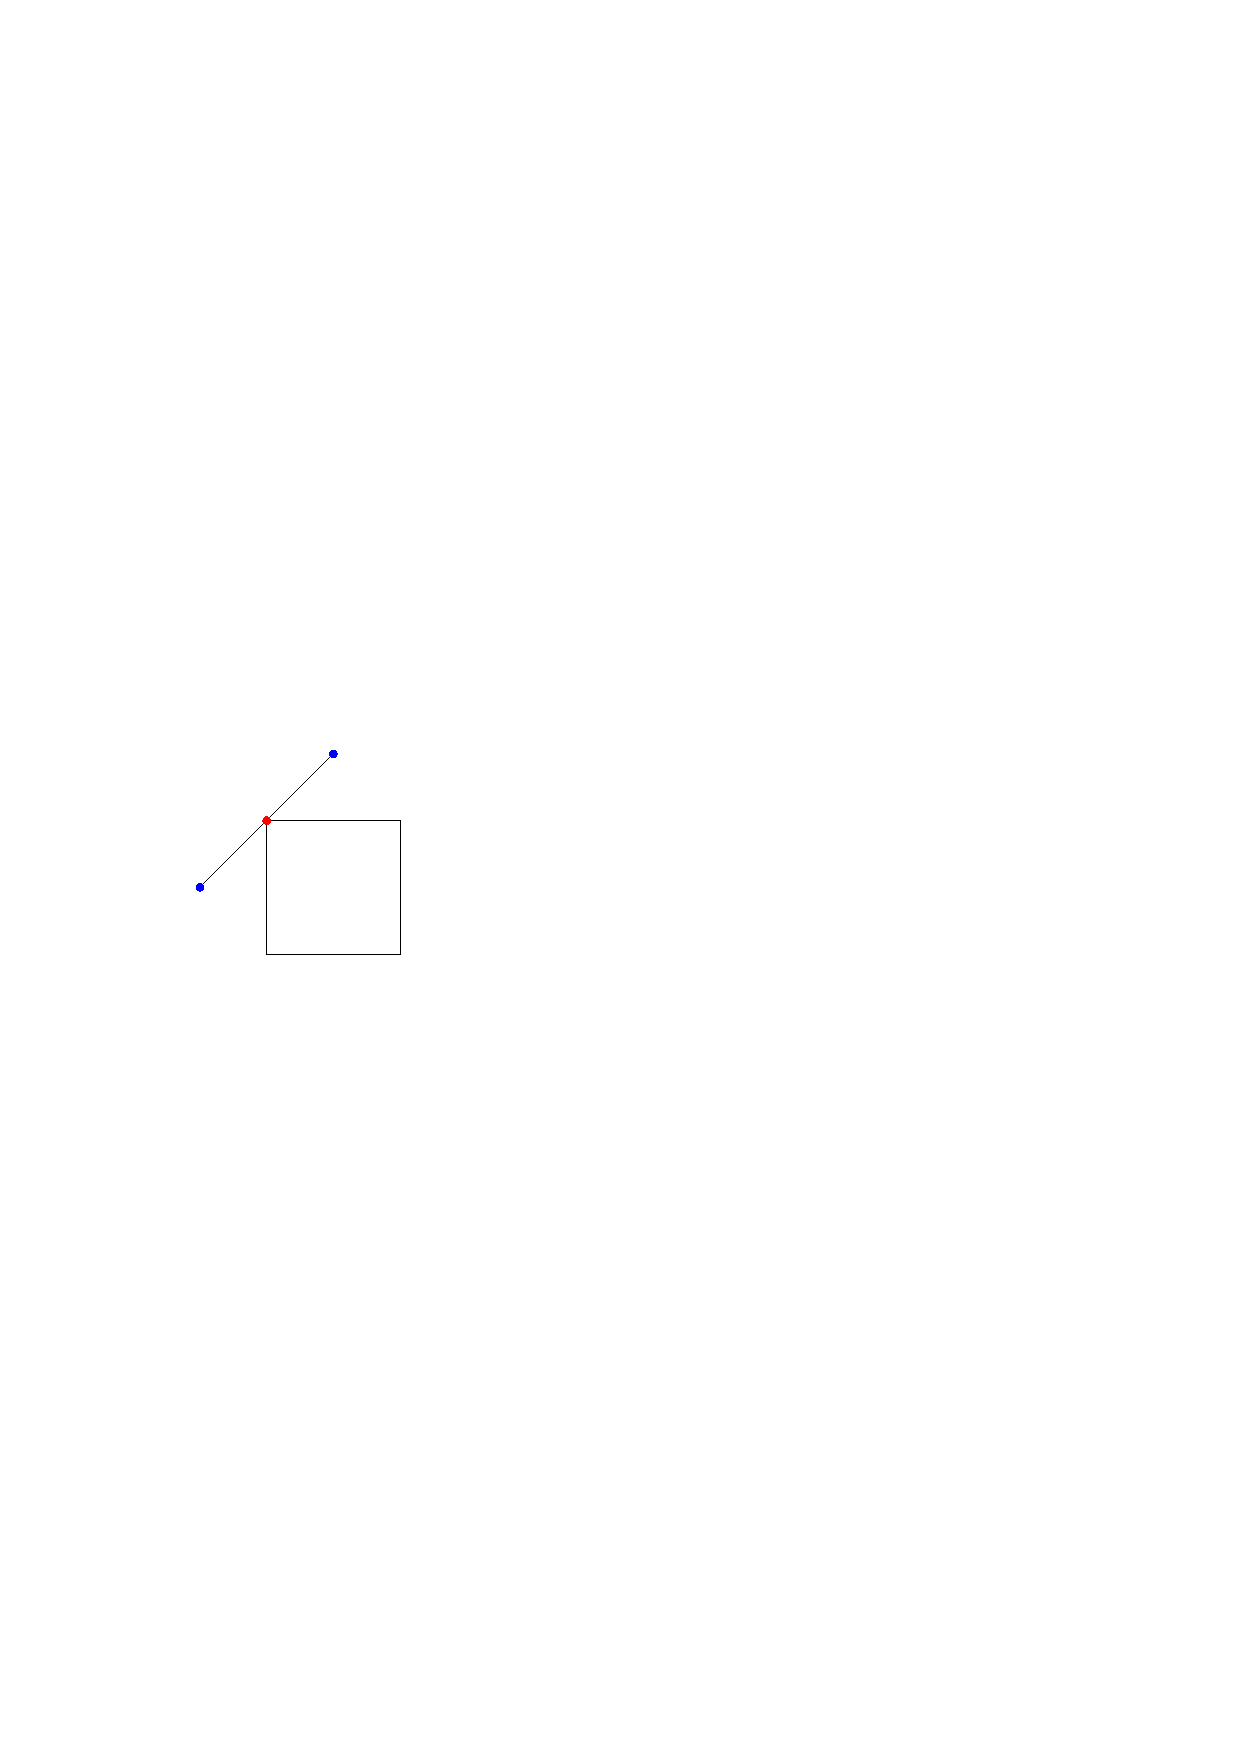
\includegraphics[width=20mm]{figures/crossFig2.pdf}} &
      \addheight{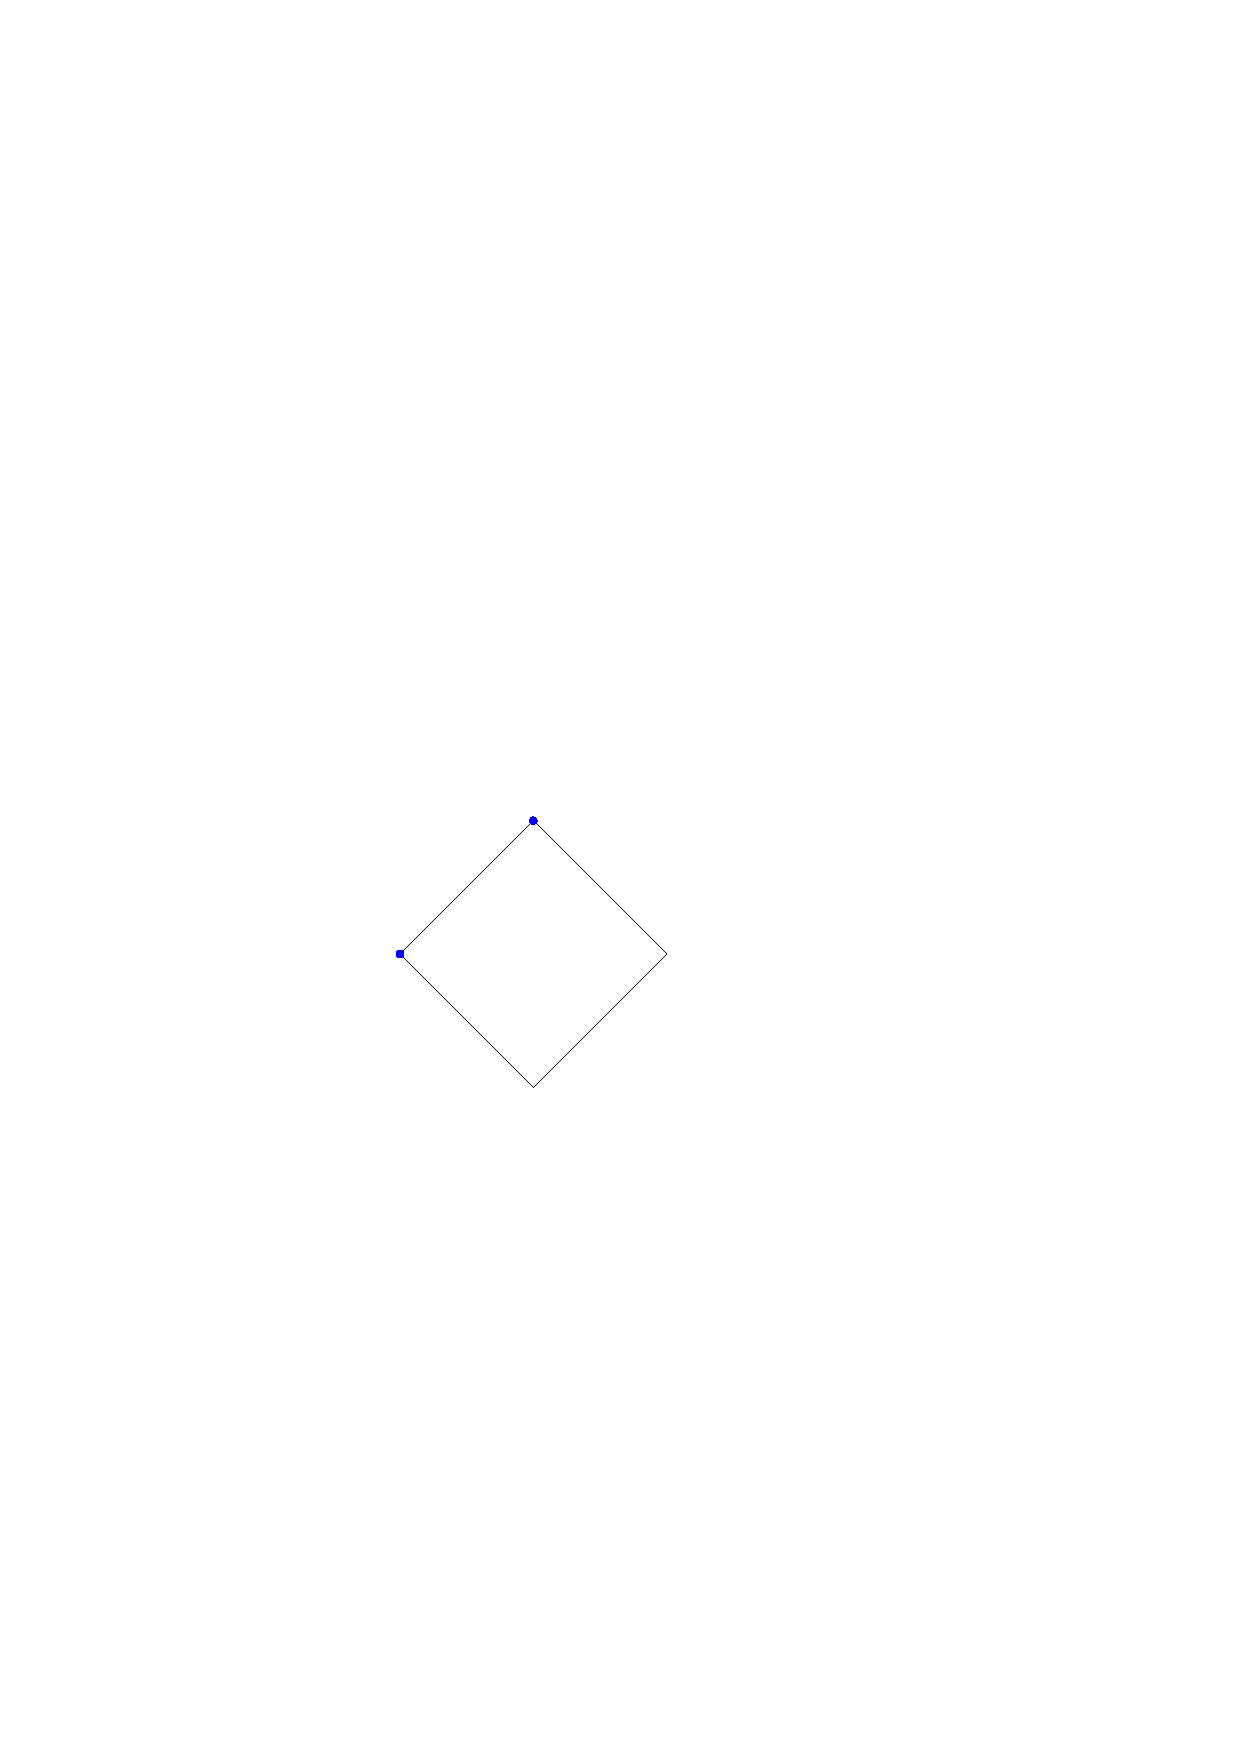
\includegraphics[width=20mm]{figures/crossFig3.pdf}} &
      \addheight{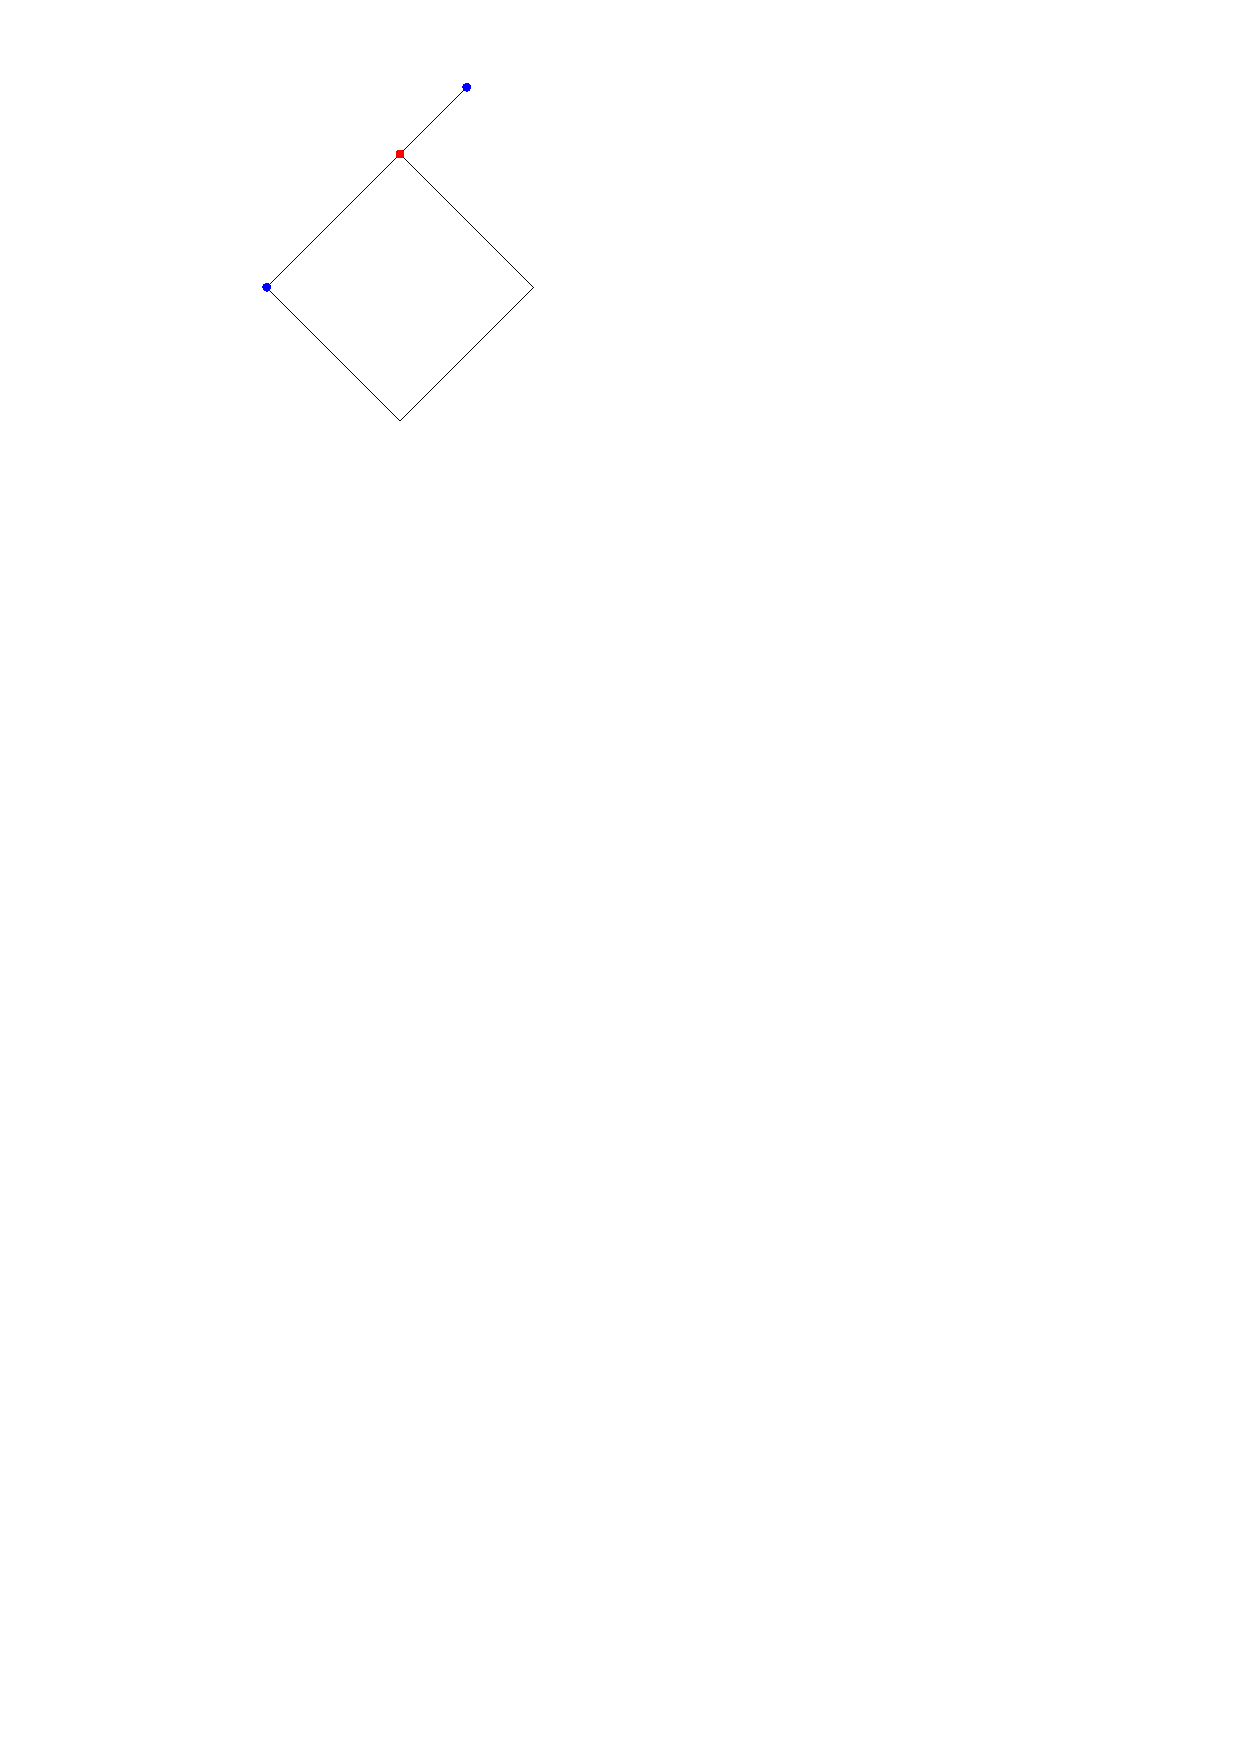
\includegraphics[width=20mm]{figures/crossFig4.pdf}} &
      \addheight{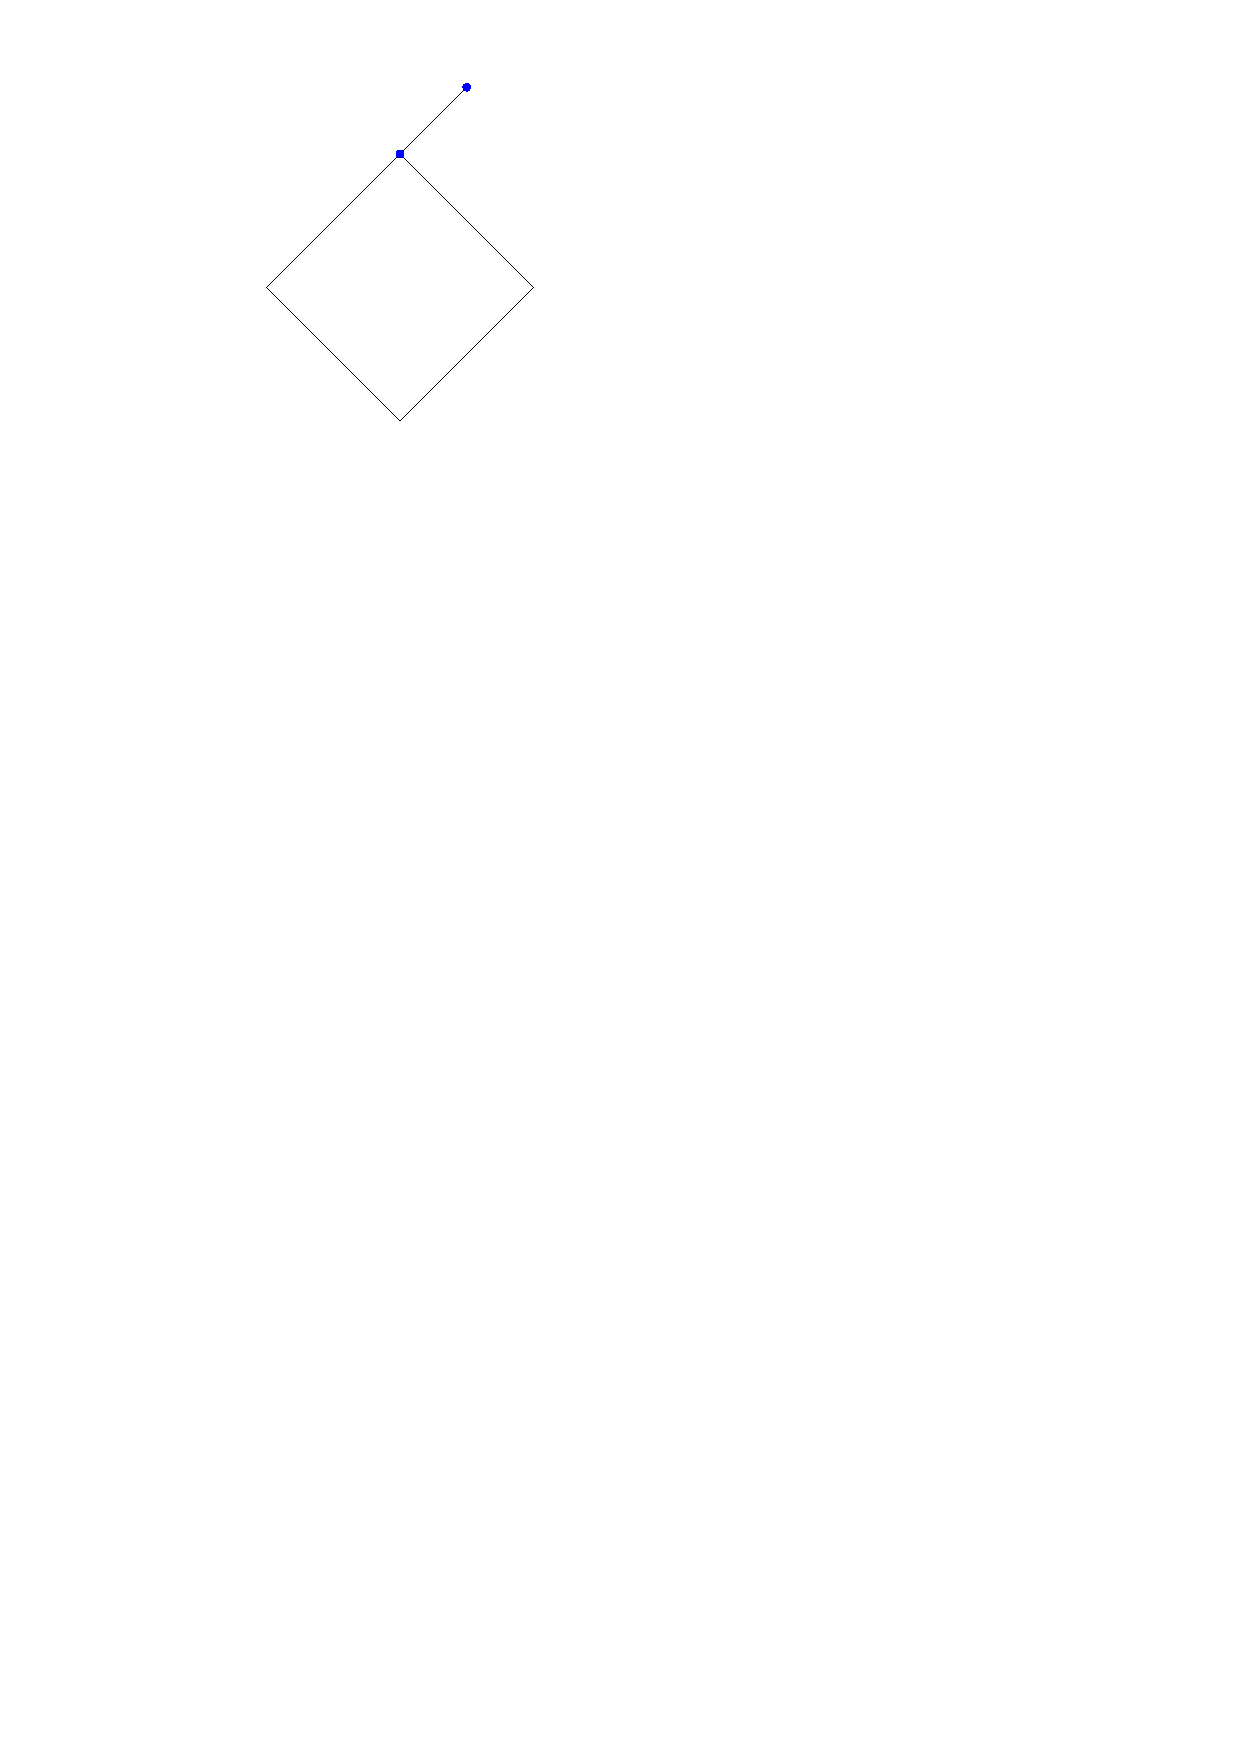
\includegraphics[width=20mm]{figures/crossFig5.pdf}} \\
      \small (a) &  (b) & (c) & (d) & (e) \\
      \hline
		\multicolumn{5}{|c|}{Intersection} \\
		\hline
      \addheight{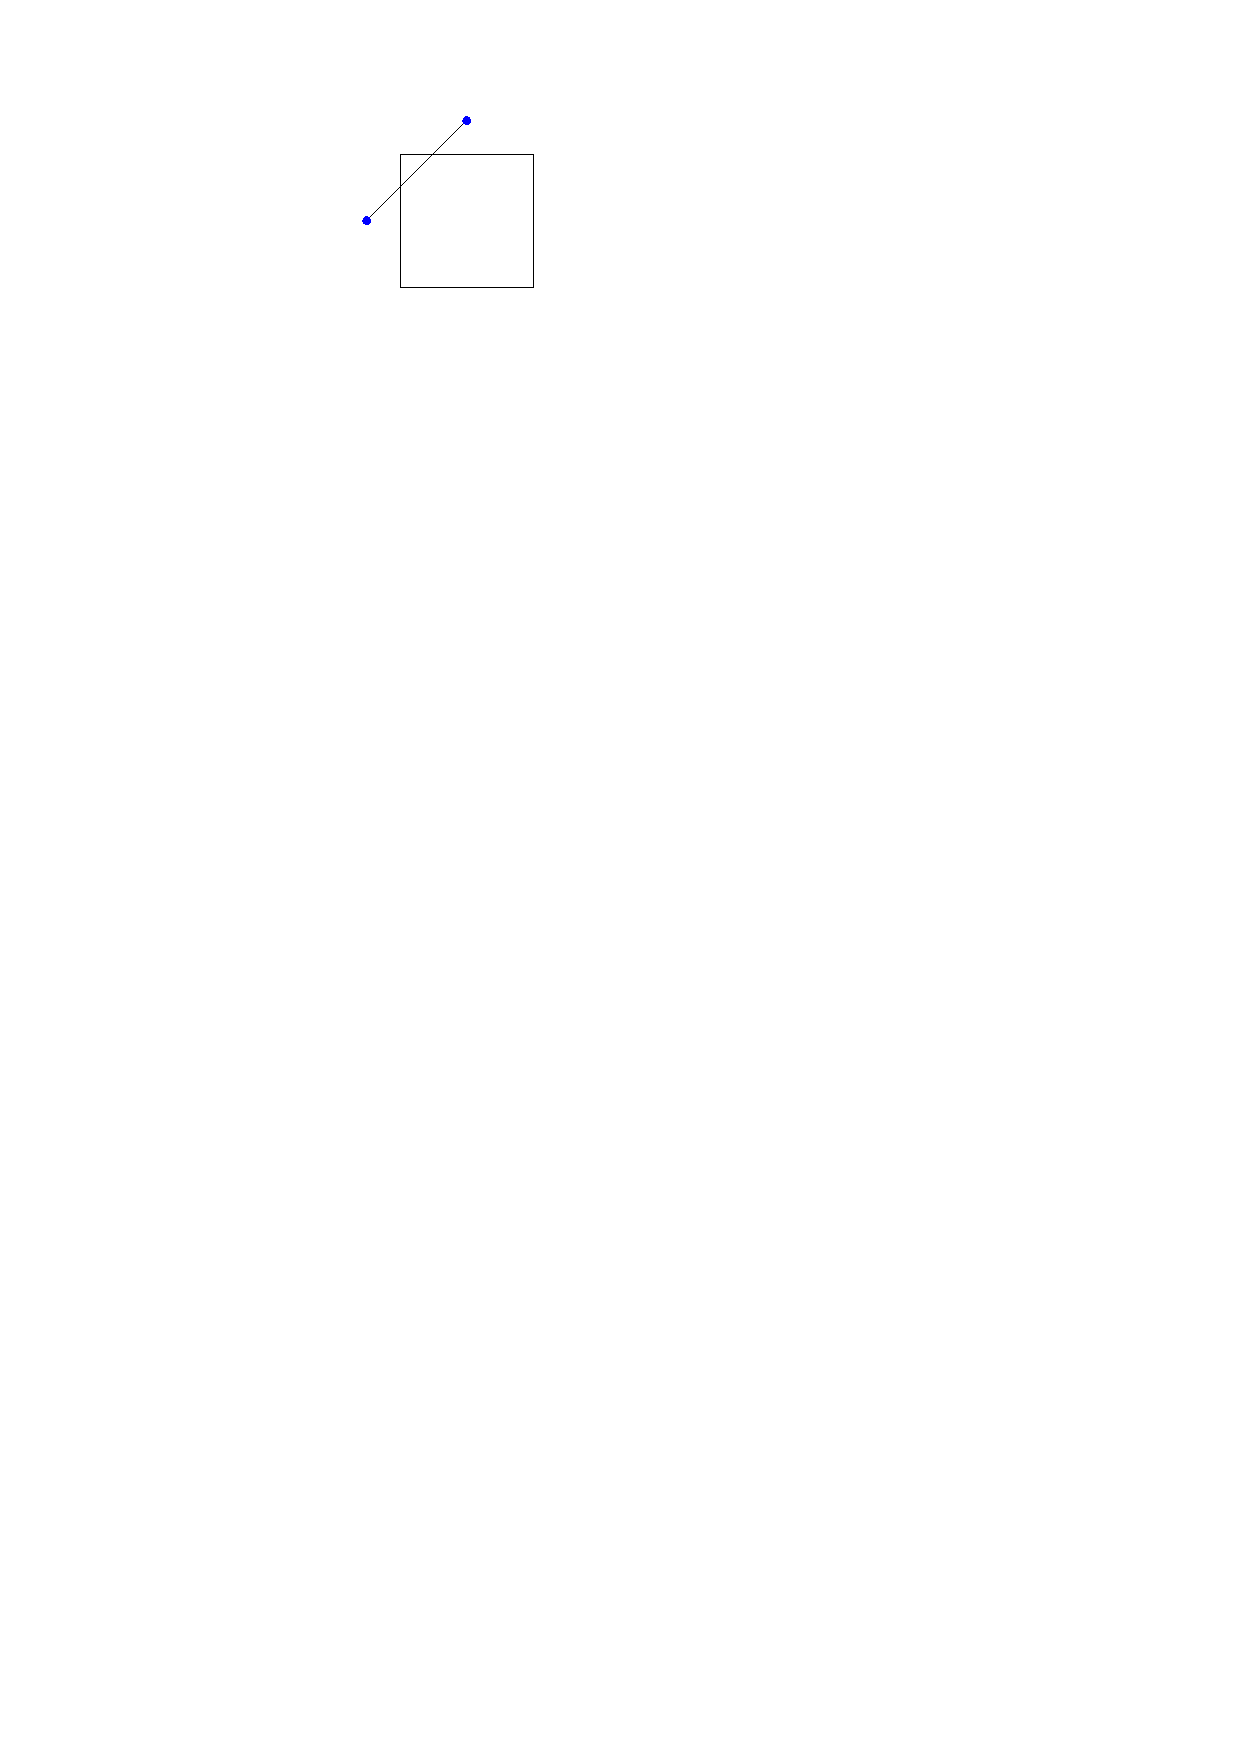
\includegraphics[width=20mm]{figures/crossFig6.pdf}} &
      \addheight{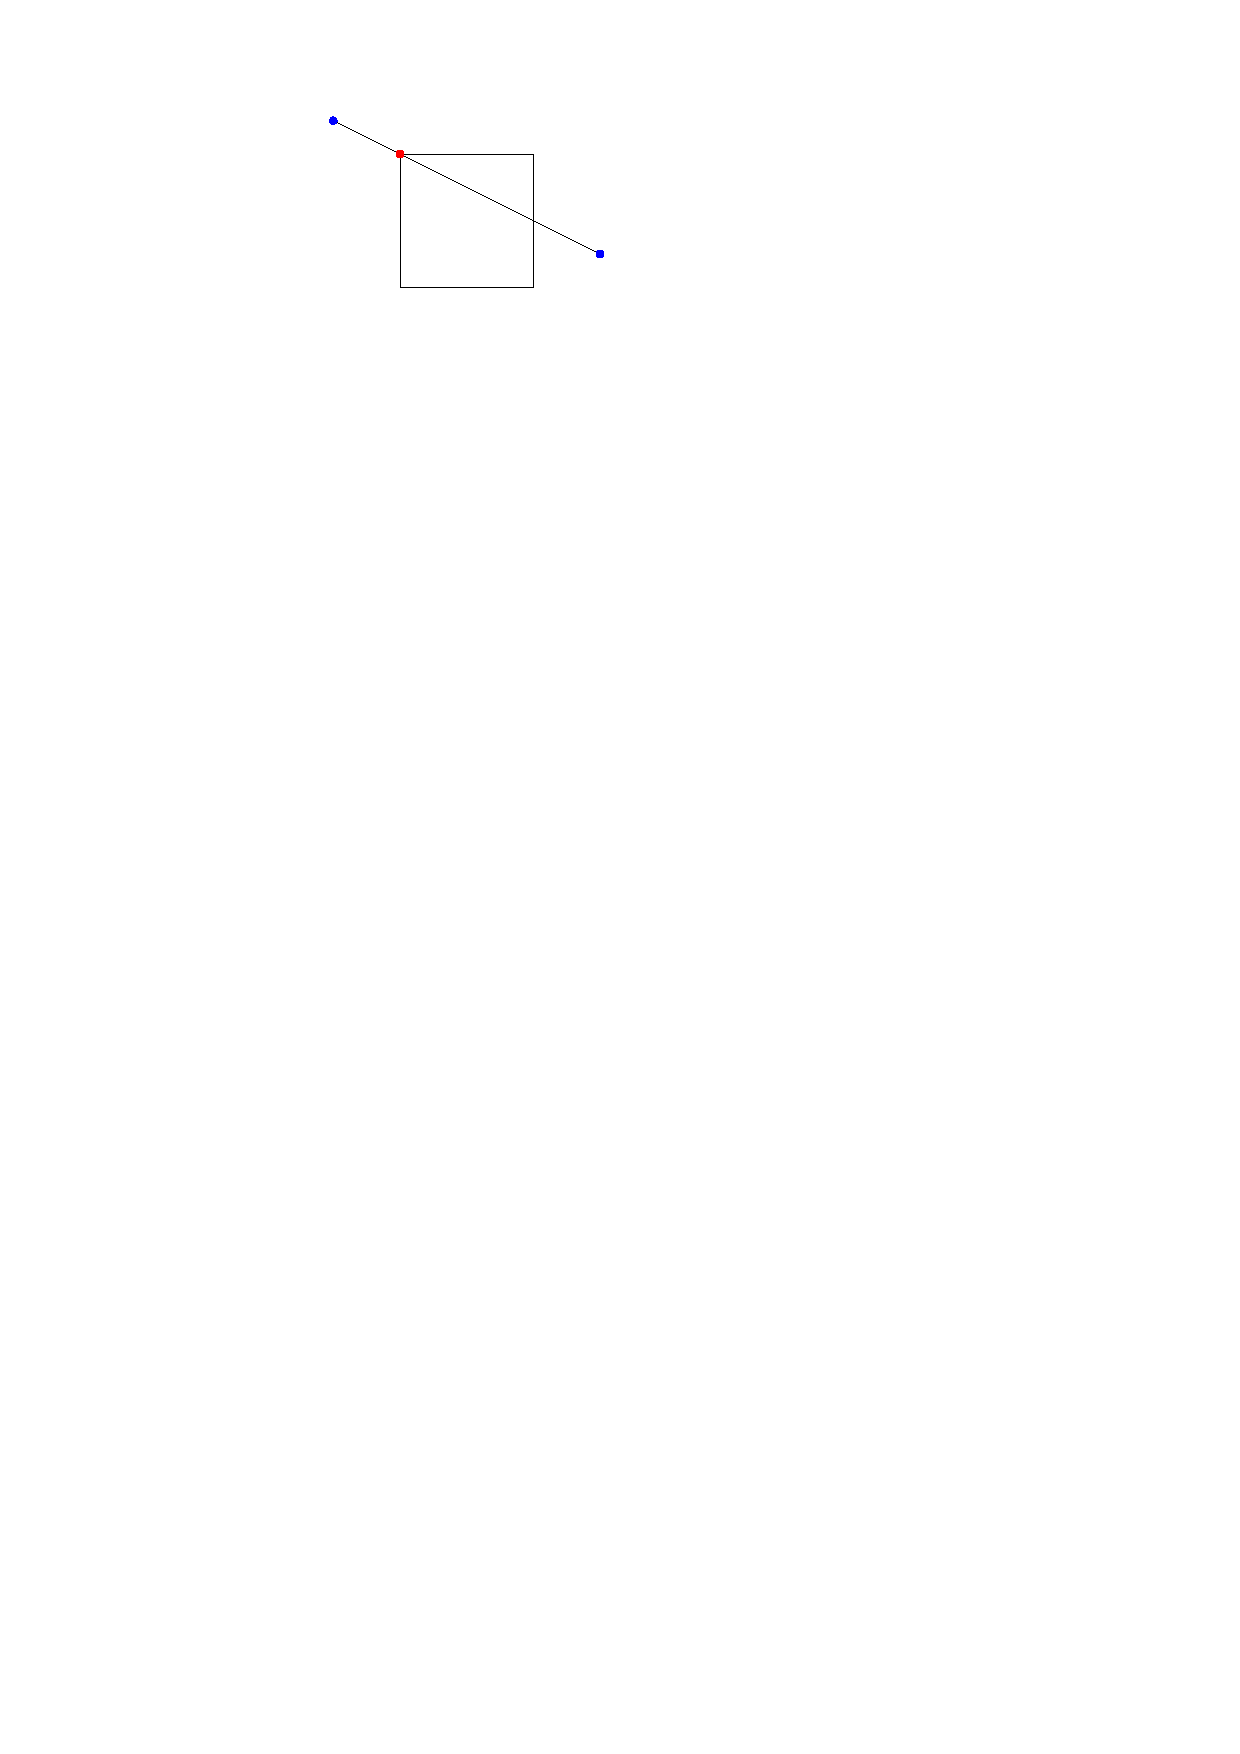
\includegraphics[width=20mm]{figures/crossFig7.pdf}} &
      \addheight{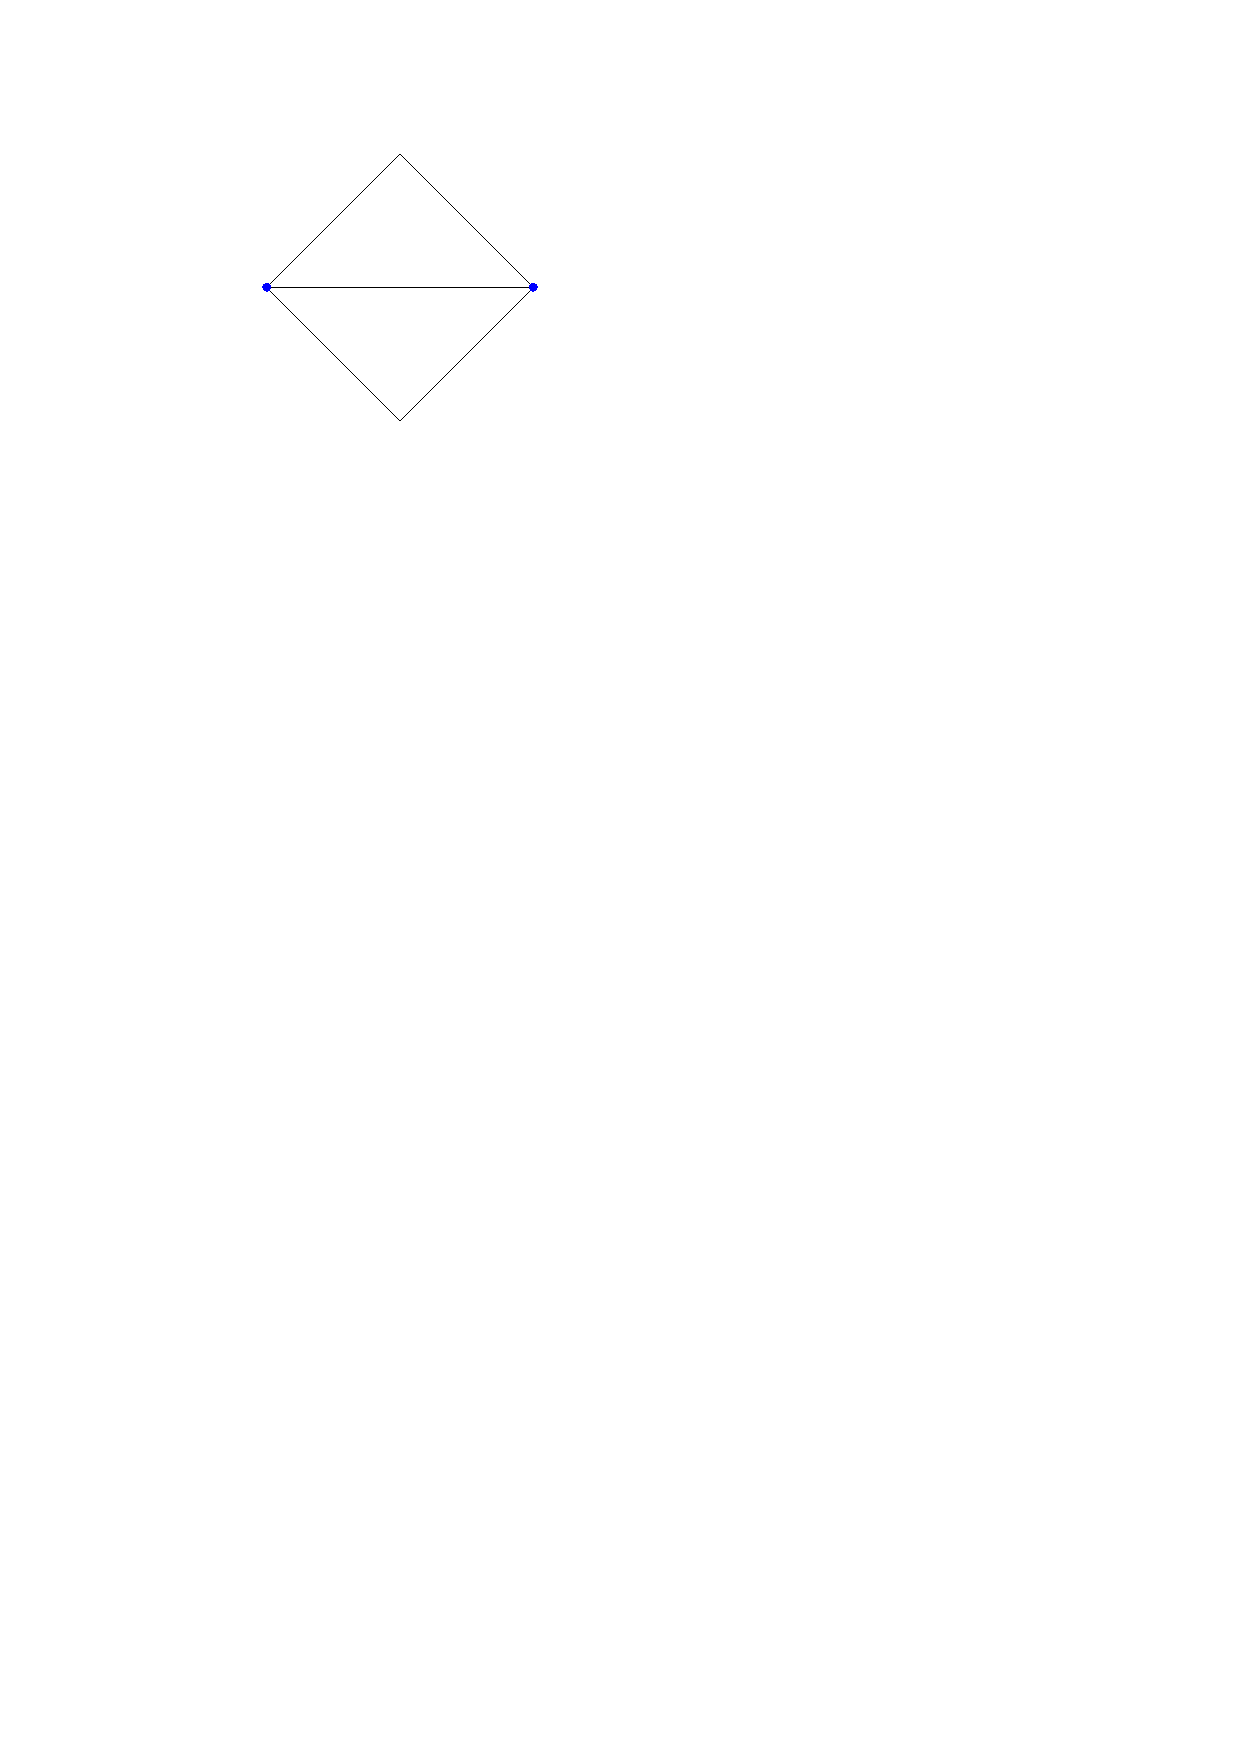
\includegraphics[width=20mm]{figures/crossFig8.pdf}} &
      \addheight{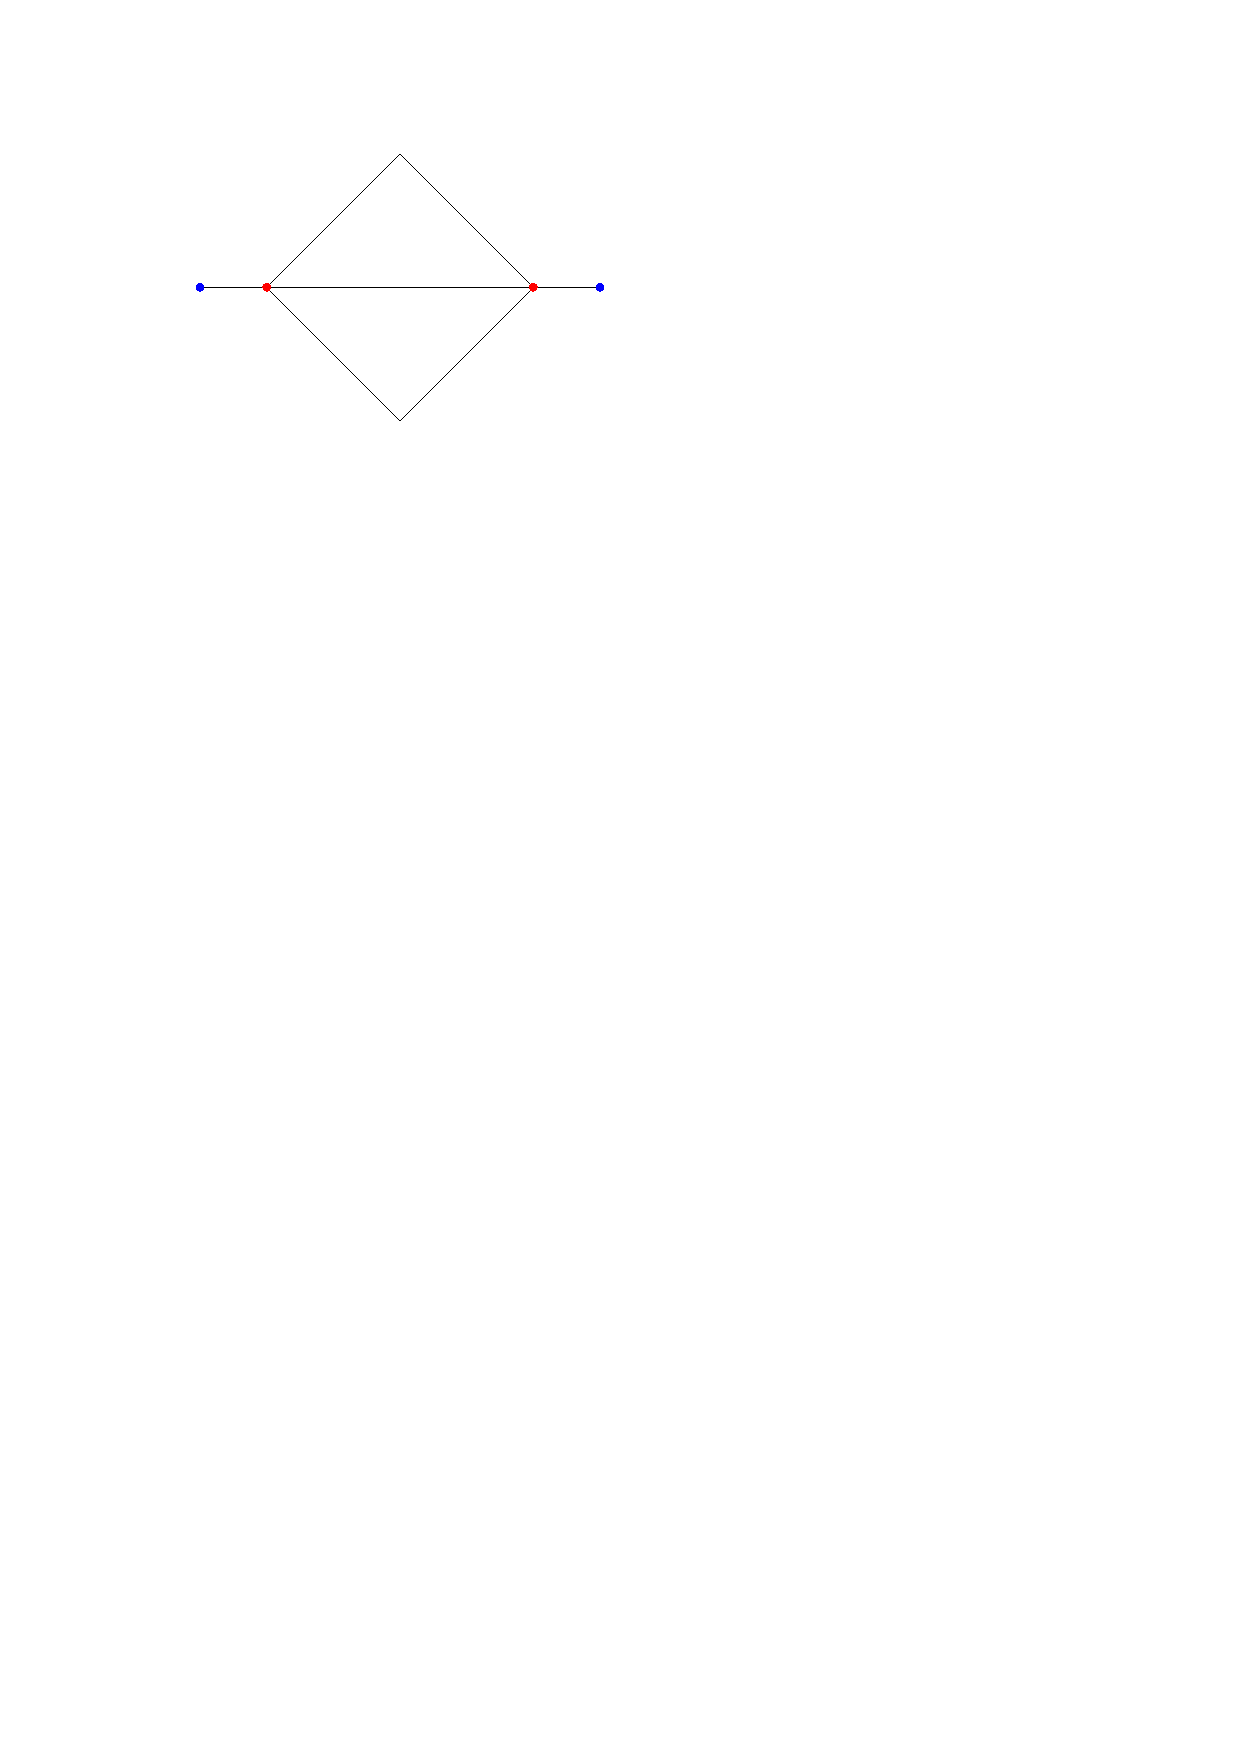
\includegraphics[width=20mm]{figures/crossFig9.pdf}} &
      \addheight{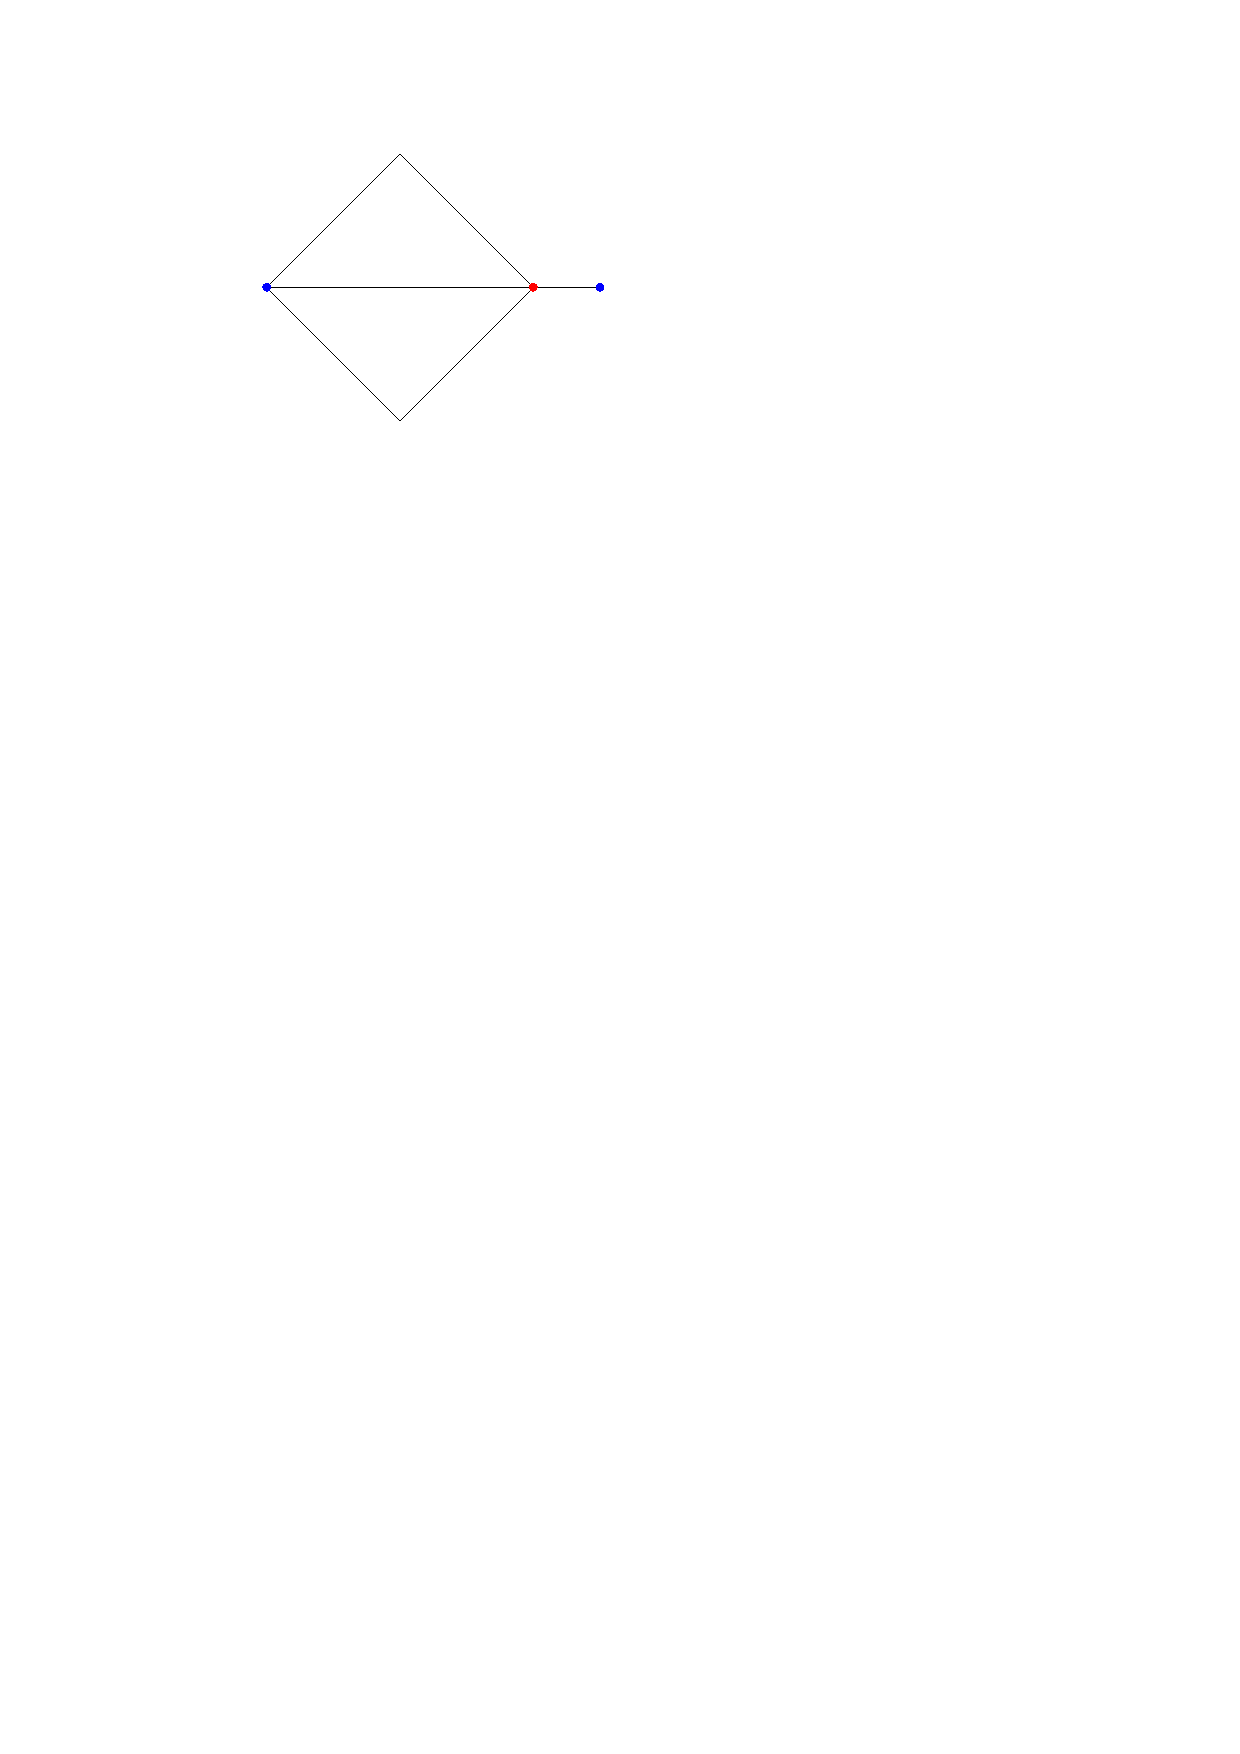
\includegraphics[width=20mm]{figures/crossFig10.pdf}} \\
      \small (f) &  (g) & (h) & (i) & (j) \\
      \hline
    \end{tabular}
    \caption{A collection of 10 different cases showing what we have 
             defined as an intersection between a polygon and a line segment}
	\label{fig:crossings}
\end{figure}

So given a polygon $O\in \mathcal{O}$, and a line segment $l$ we want to determine
weather $l$ crosses the polygon $O$. We start by making the list of points into
a list of line segment $O'=(p_1,p_2),(p_2,p_3),\dots,(p_{i-1},p_i)$.  Then we
observe that if a line segment crosses a line segment of a polygon, it counts
as a crossing (cases f and g). The other three cases of crossing (cases h, i
and j) all have that in common that the line segment crosses four end points
from the polygon. So we say it is not allowed to cross four points in of
a polygons line segments. The problem is that it makes (cases a, c
and d) illegal. But fortunately they all have that in common that they are collinear 
(they lie on a common line) with a line segment of the polygon, so the
algorithm is as follows:

\begin{enumerate}
	\item if a line segment $l_1$ crosses another line segment $l_2$ of a polygon it 
	      crosses the polygon
	\item if a line segment has four points in common with the polygon it crosses the
		  polygon, unless the line segment is collinear with a line segment of the
		  polygon 
\end{enumerate}

This lead us to the following algorithm
\begin{algorithm} 
	\caption{NumberOfCrossings($l,O$)}
	\begin{algorithmic}[1] 
		\State{result=0}
		\ForEach{$o \in O$}
			\State{counter$=0$}
			\ForEach {$l' \in o$}
				\State{result$=$crosses$(l',l)$}
				\If{result==-1}
					\State{counter$=0$}
					\State{\textbf{Break}}
				\ElsIf{result==0}
					\State{counter=counter+1}
				\Else
					\State{counter=4}
					\State{\textbf{Break}}
				\EndIf
			\EndFor
			\If{$counter>4$}
				\State{result=result+1}
			\EndIf
		\EndFor
		\Return{result}
	\end{algorithmic}
\end{algorithm}

\subsection{Crosses}
To make a crosses function, we need a right turn function. Consider three
points $p_1,p_2,p_3$ in the plane, make a line that goes through $p_1$ and $p_2$. 
Now if we stand at point $p_1$ and look in the direction of $p_2$ will $p_3$, if $p_3$
doesn't lie on the same line as $p_1$ and $p_2$ will it be on the
right or the left of the line. Let $p_i.x$ and $p_i.y$ denote the x-coordinates
and y-coordinates respectively. To find out whether the three points form a right turn, 
a left turn or are collinear we make the following two vectors.

\begin{align*}
	v_1 &=p_2-p_1 = \langle p_2.x-p_1.x,p_2.y-p_1.y\rangle\\
	v_2 &=p_3-p_1 = \langle p_3.x-p_1.x,p_3.y-p_1.y\rangle
\end{align*}
Lets denote $v_1 = \langle a,b\rangle$ and $v_2 = \langle c,d\rangle$
(see Figure \ref{fig:rightturn_a})

\subsection{Right turn}

\begin{figure}[H]
    \centering
	\begin{subfigure}{.7\textwidth}
		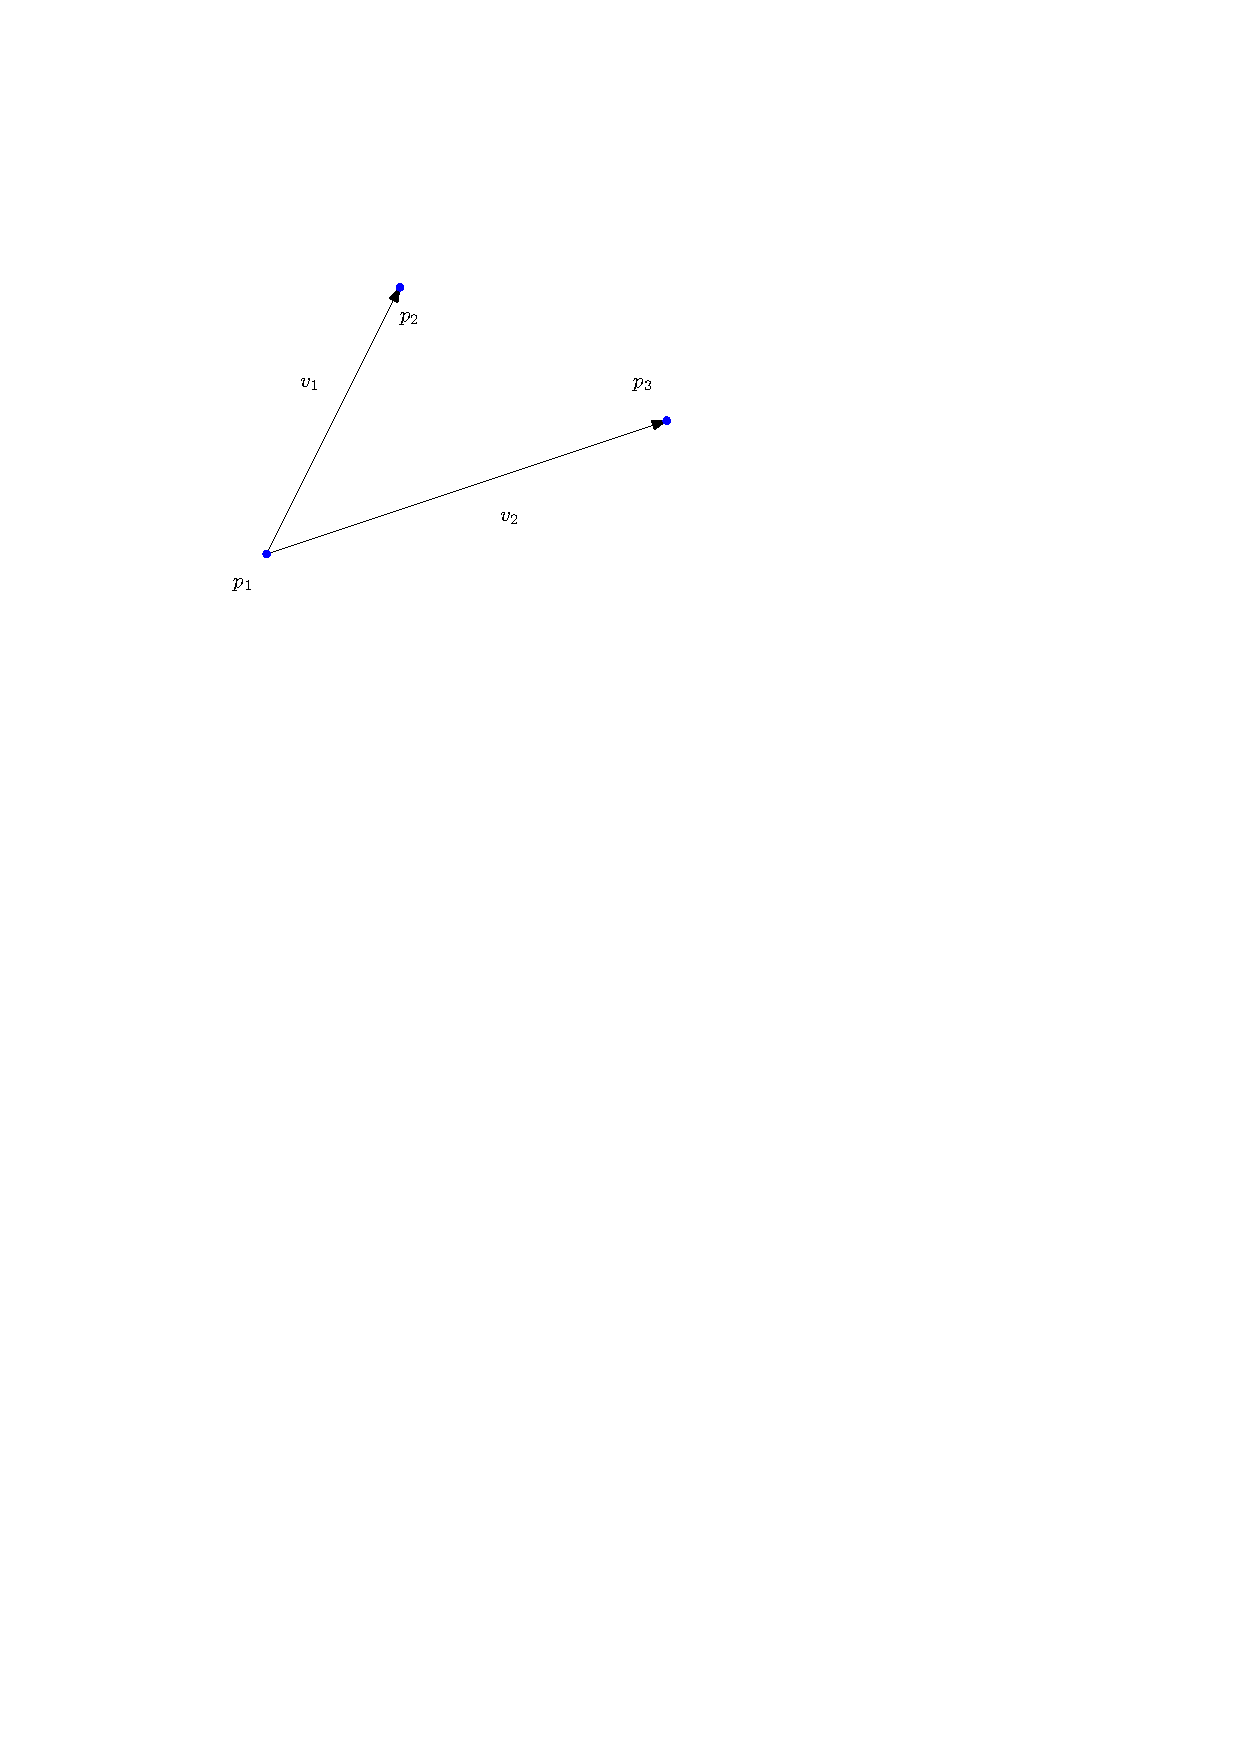
\includegraphics[width=.5\textwidth]{figures/rightturn1.pdf}
		\caption{}
		\label{fig:rightturn_a}
	\end{subfigure}
	\caption{A right turn formed by three points}
    %
	\begin{subfigure}{.7\textwidth}
		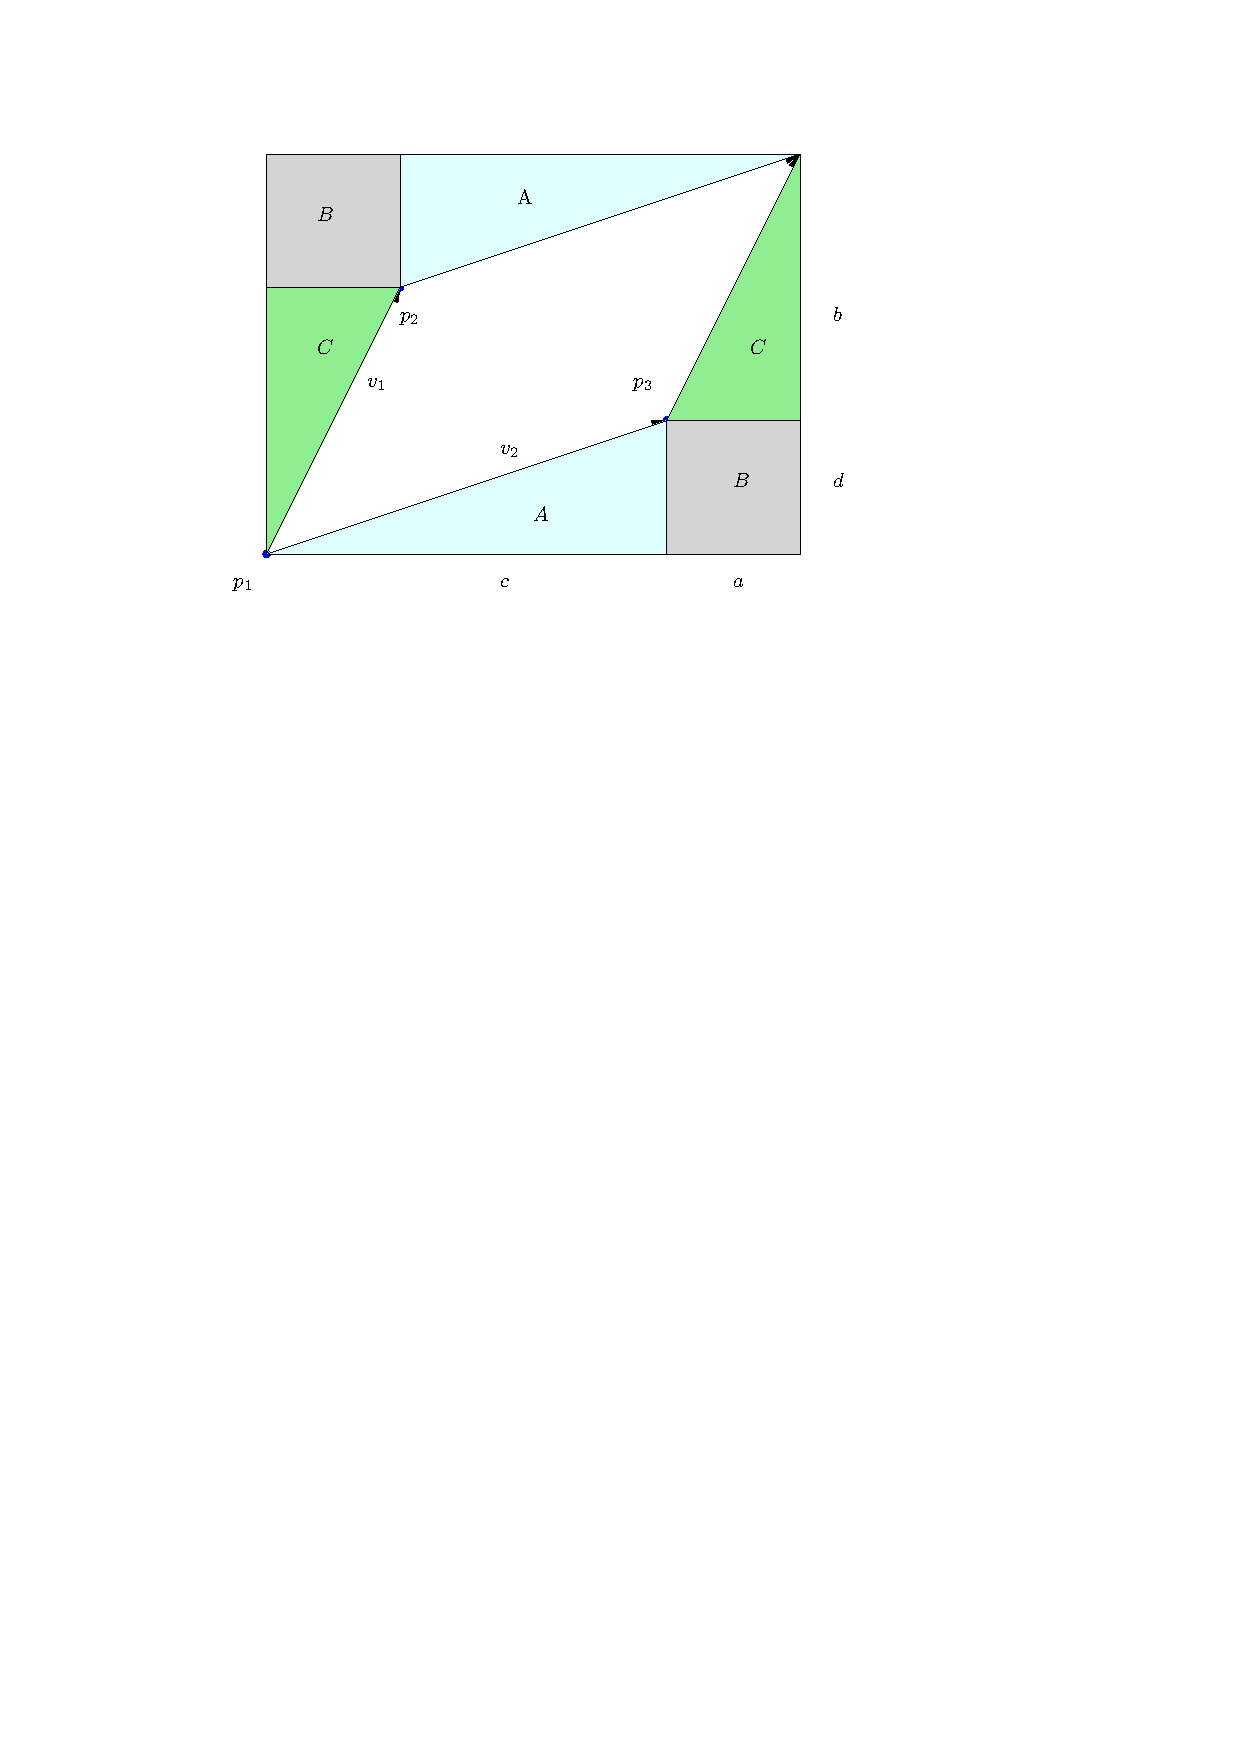
\includegraphics[width=8cm]{figures/rightturn2.pdf}
		\caption{}
		\label{fig:rightturn_b}
	\end{subfigure}
	\caption{Area are of a parallelogram given by two vectors}
\end{figure}

We claim that we can calculate the turn by calculating the signed area of the
parallelogram spanned by the two vectors. The area of their parallelogram can
be calculated as follows: calculate the area of the big rectangle, and take the
two small triangles and the little square and subtract that area.

\begin{align}
	\text{area} &= (a+c)(d+b)-2A-2B-2C\nonumber\\
							&=ad+ab+cd+bc-cd-2ad-ab\nonumber\\
							&=bc-ad \nonumber\\
							&=(p_2.y-p_1.y)(p_3.x-p_1.x)-(p_2.x-p_1.x)(p_3.y-p_1.y)\label{form:rightturn}
\end{align}

Now we claim that the area between these two vectors is positive if the
three points form a right turn, and negative if they form a left turn. We show
that by an example (see figure \ref{rightturn3})

Given our formula (formula \ref{form:rightturn}) we get that the $q_1,q_3,q_2$ area is

\begin{align*}
	&(q_3.y-q_1.y)(q_2.x-q_1.x)-(q_3.x-q_1.x)(q_2.y-q_1.y)\\ 
	= &(2-0)(-1-0)-(0-0)(1-0)\\
	= & 2\cdot (-1)-0\cdot1\\
	= & -2-0\\
	= & -2
\end{align*}
And the area of $q_1,q_3,q_4$ is
\begin{align*}
	&(q_3.y-q_1.y)(q_4.x-q_1.x)-(q_3.x-q_1.x)(q_4.y-q_1.y)\\ 
	= &(2-0)(1-0)-(0-0)(1-0)\\
	= &(2\cdot 1 - 0\cdot 1\\
	= &2-0\\
	= &2
\end{align*}

\begin{figure}[H]
    \centering
	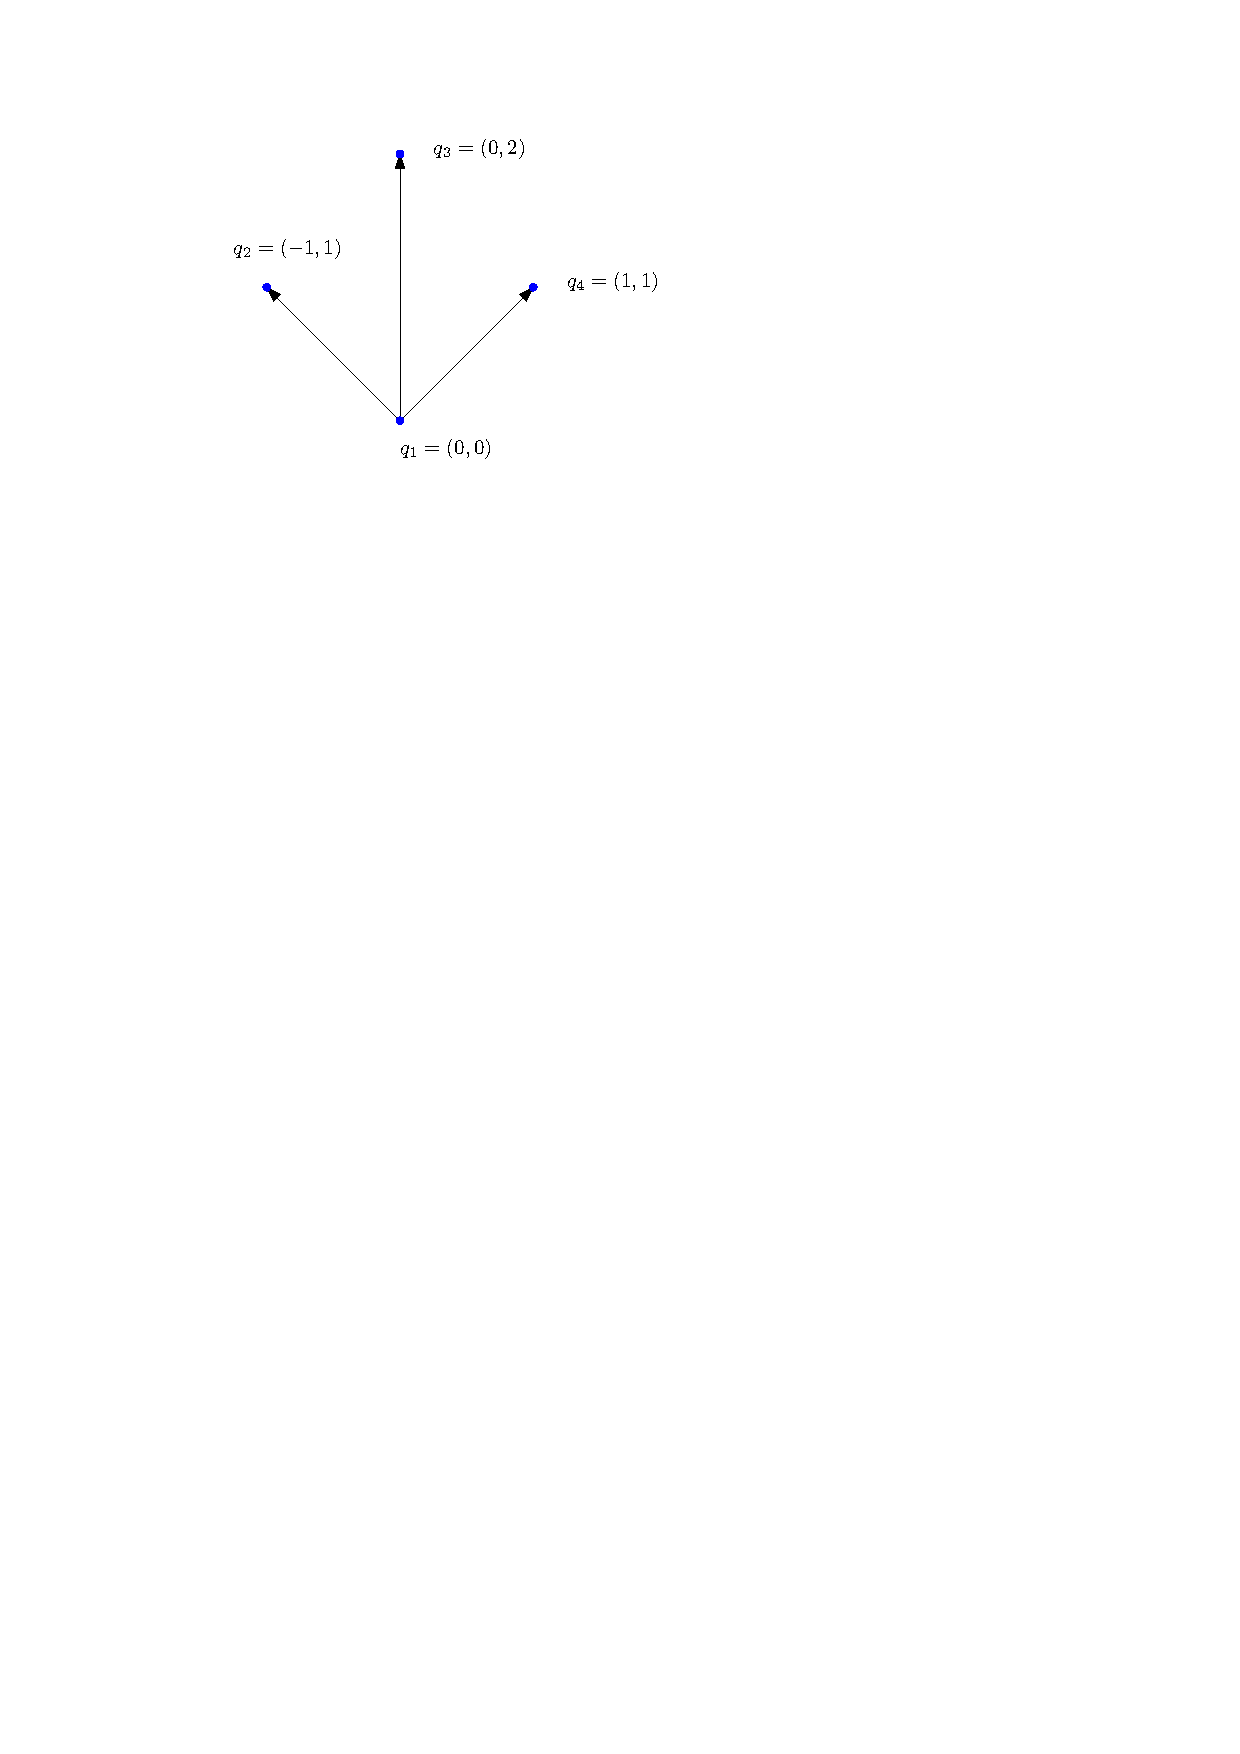
\includegraphics{figures/rightturn3.pdf}
	\caption{Right turn example}
    \label{rightturn3}
\end{figure}

So the function for calculating a right turn is

\begin{algorithm} 
	\begin{algorithmic}[1] 
		\State \Return $(p_2.x-p_1.x)(p_3.y-p_1.y)-(p_2.y-p_1.y)(p_3.x-p_1.x)$
	\end{algorithmic}
	\caption{rightTurn($p_1,p_2,p_3$)}
\end{algorithm}

This function will return a negative number if the three points make a left
turn, a positive number if it is a right turn and 0 if the three points are on
a line.

\subsection{Crossing of two line segments}

\begin{figure}[H]
	\minipage{0.32\textwidth}
		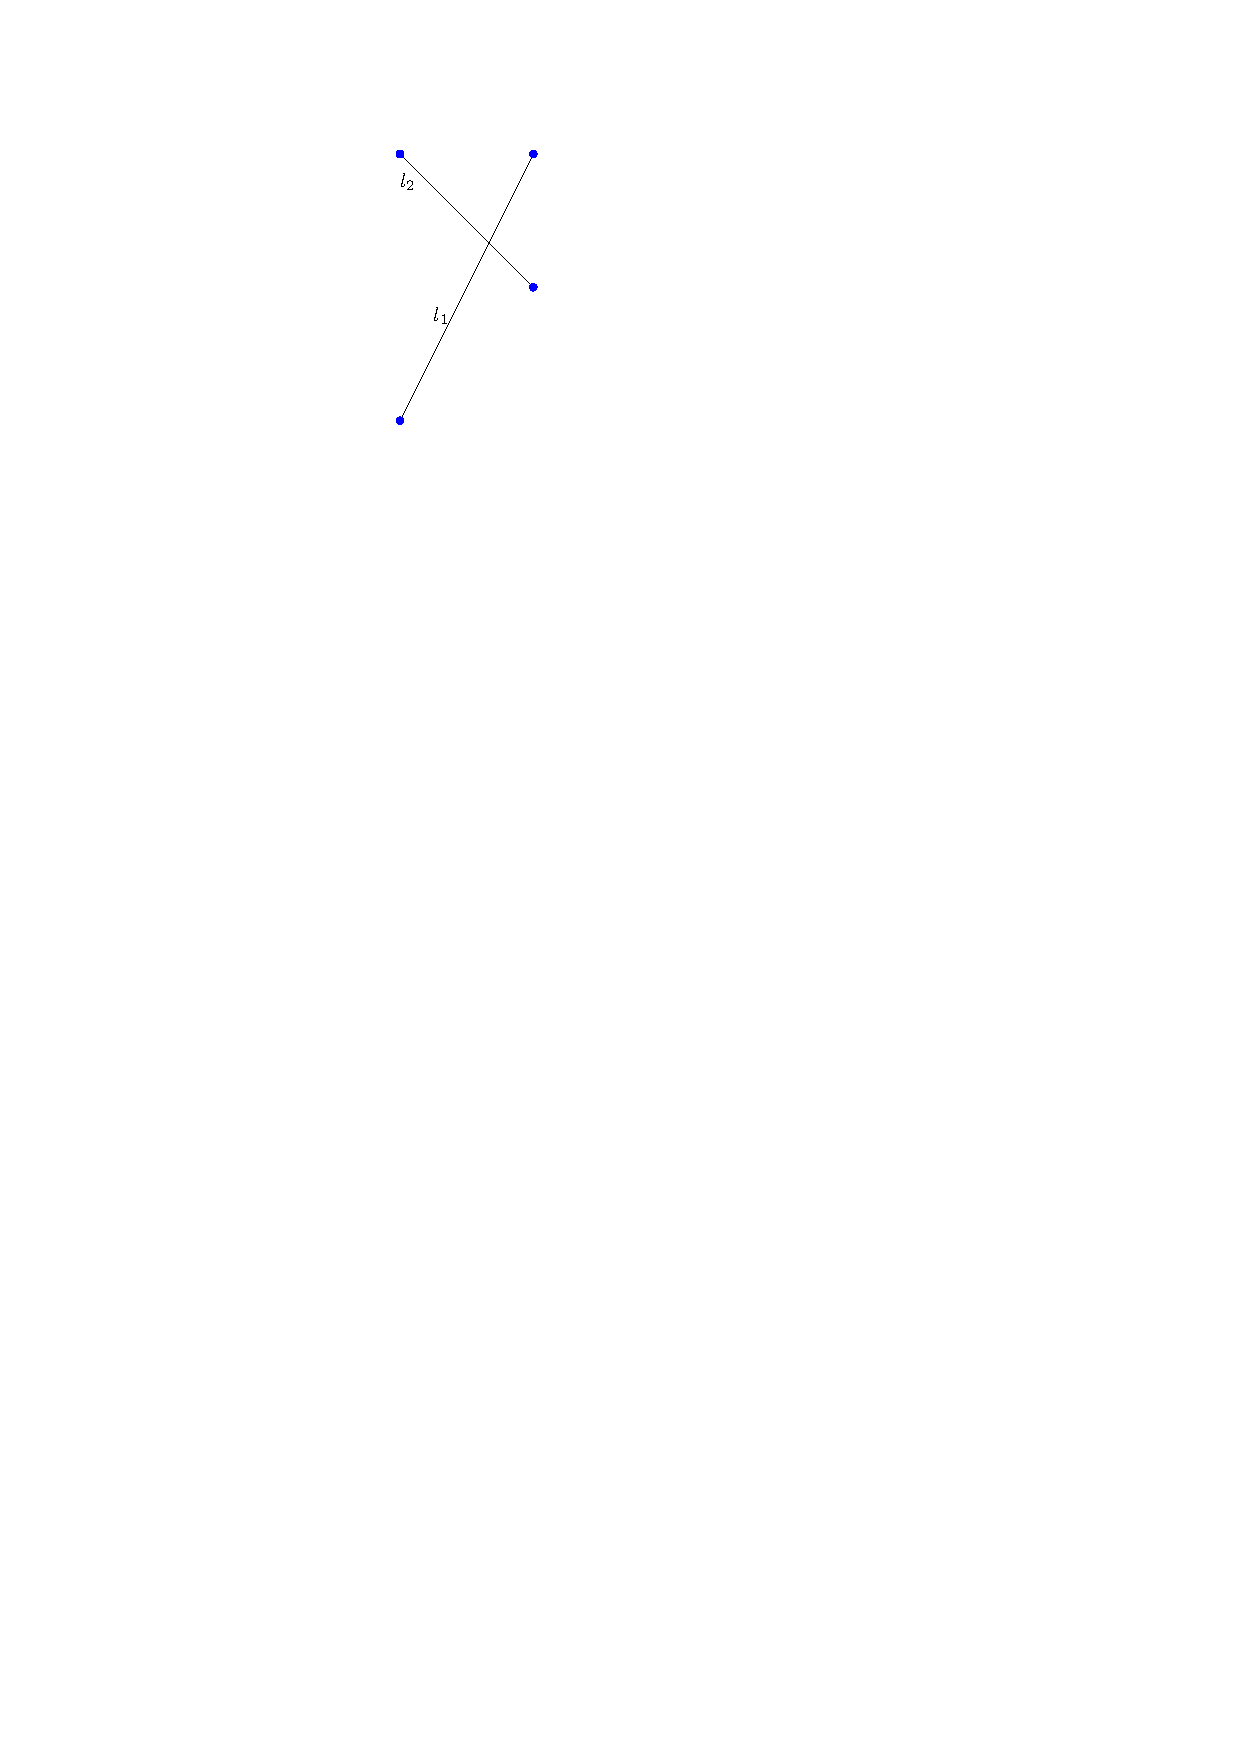
\includegraphics[width=2cm]{figures/crosses.pdf}
		\caption{Two lines crossing}
		\label{fig:crosses_a}
	\endminipage\hfill
	\minipage{0.32\textwidth}
		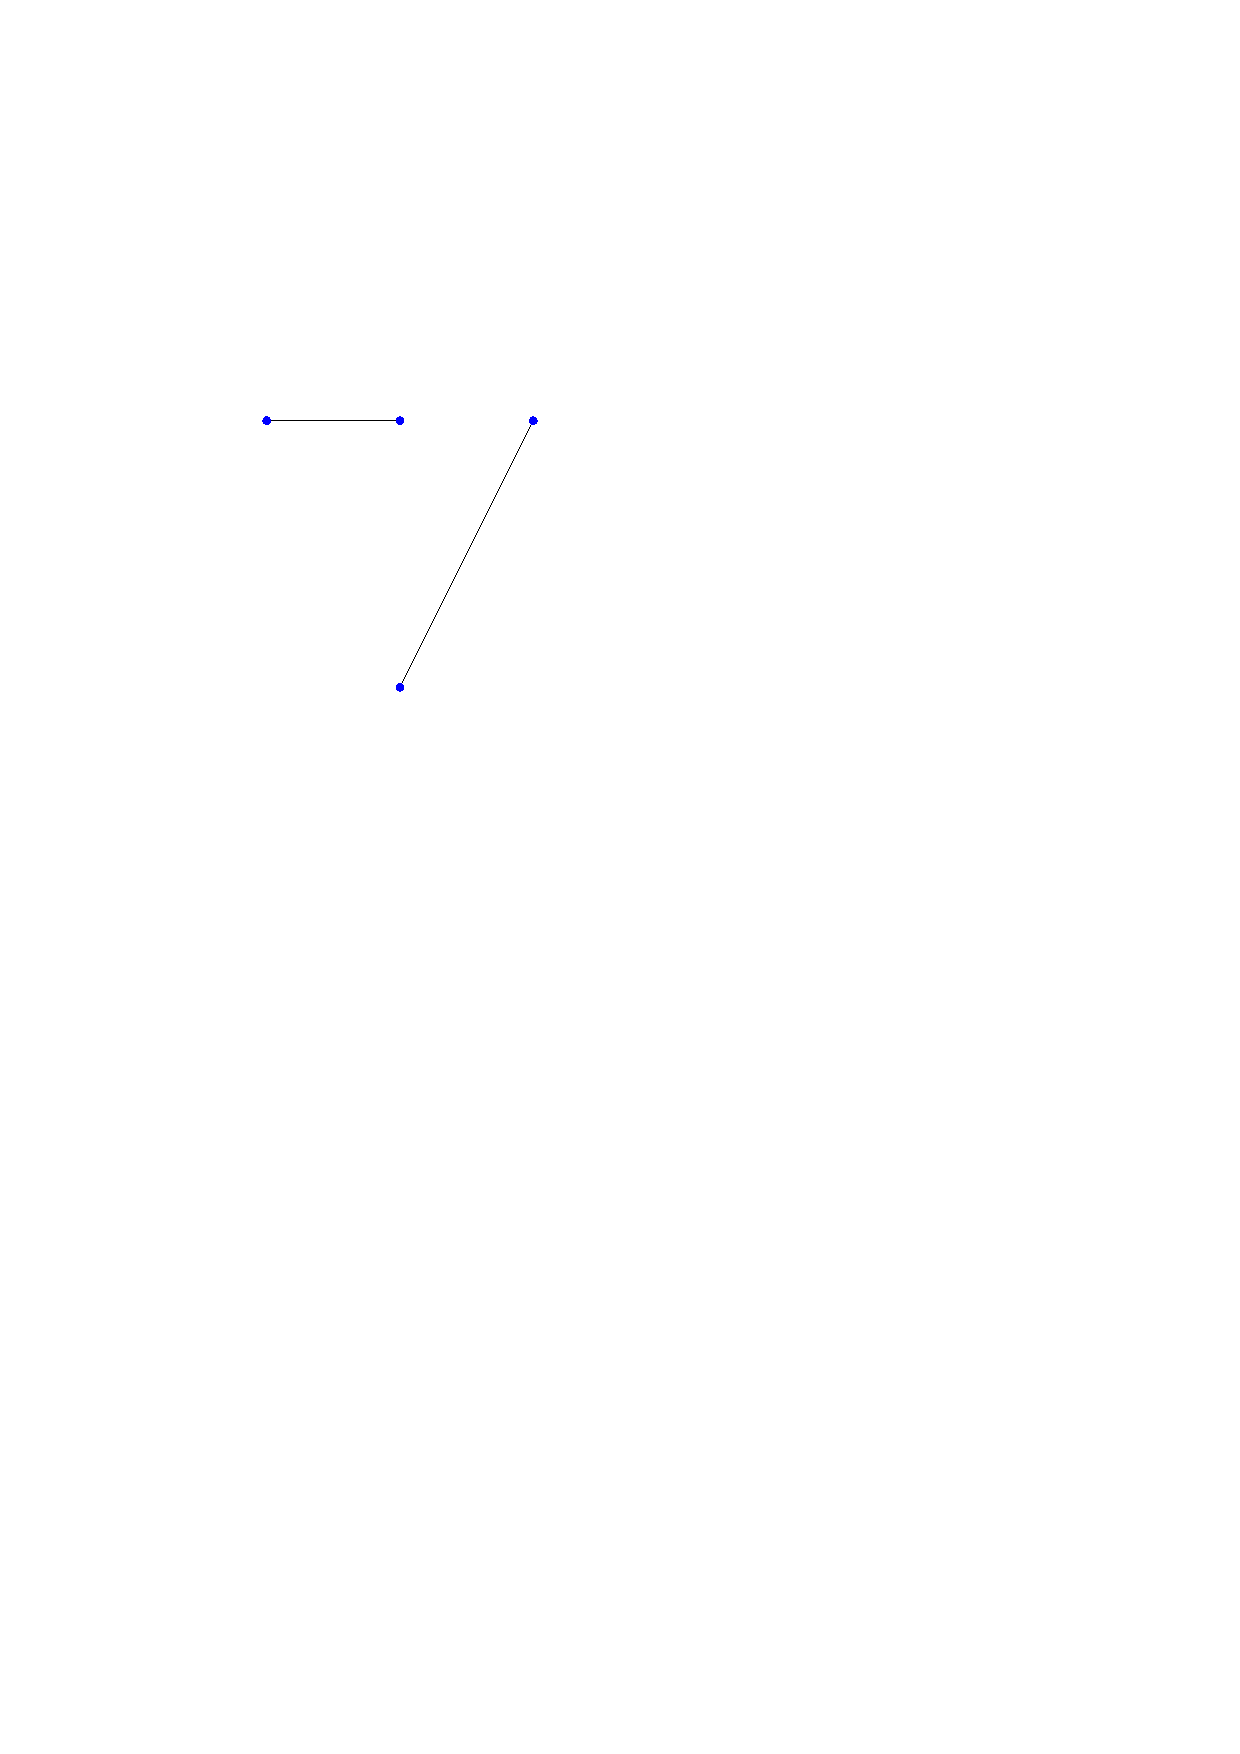
\includegraphics[width=3cm]{figures/crosses1.pdf}
		\caption{Two line which does not cross}
		\label{fig:crosses_b}
	\endminipage\hfill
	\minipage{0.32\textwidth}
		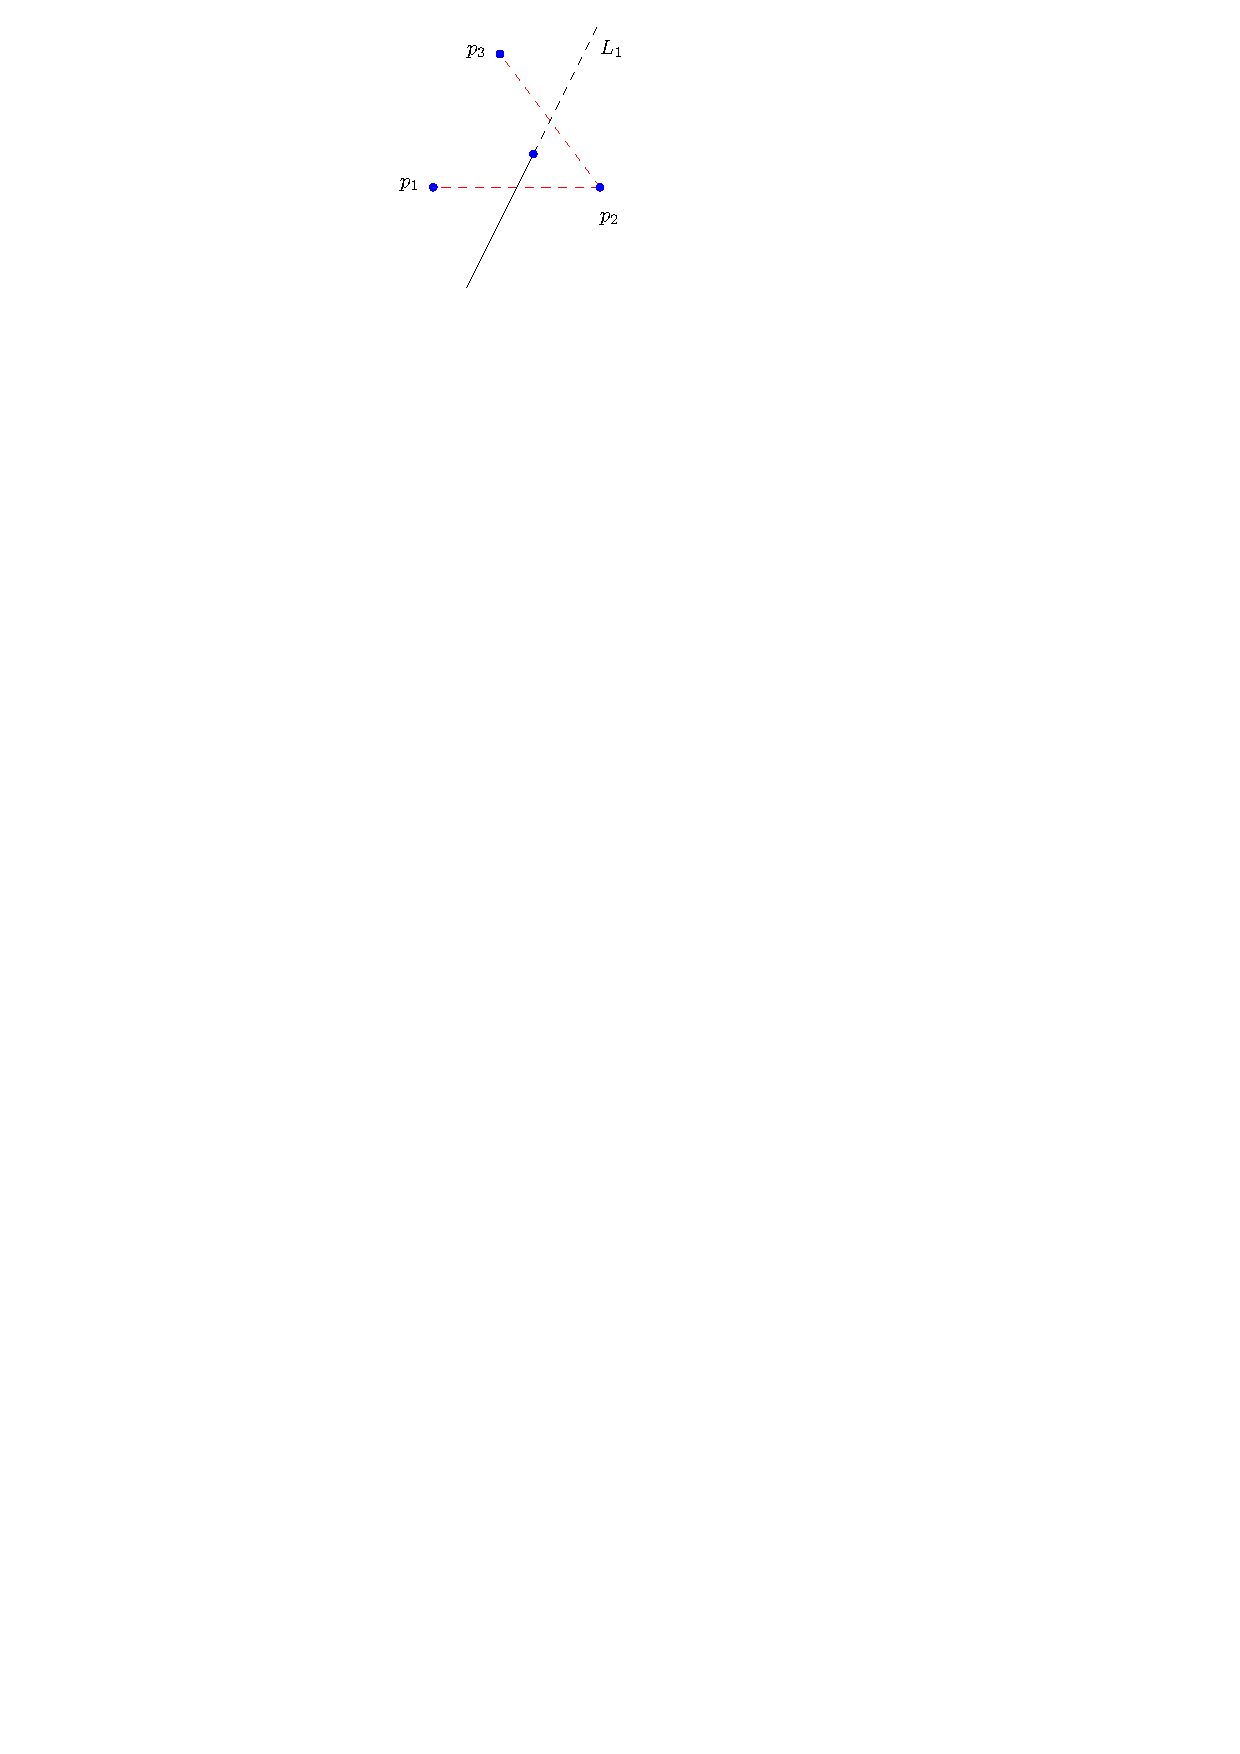
\includegraphics[width=3cm]{figures/crosses2.pdf}
		\caption{$\overline{p_1p_2}$ passes both tests of \ref{lemma:crosses}, while $\overline{p_2p_3}$ only passes one}
		\label{fig:crosses_c}
		\endminipage\hfill
\end{figure}

\begin{Lemma} \label{lemma:crosses}
    Given two line segments, $l_1$ and $l_2$ we can decide whether they cross
    by first checking if the two end points of $l_2$, namely $l_2.p$ and $l_2.q$, 
    lie on separate sides of the line which is collinear to $l_1$. Should this be
    the case, we do a similar check for $l_2$ on $l_1$. Should both cases be true
    we know $l_1$ crosses $l_2$, see figure \ref{fig:crosses_a}.
\end{Lemma}

\begin{proof}
Let $L_1$ and $L_2$ denote the lines collinear to $l_1$ and $l_2$ respectively.
	If both the end points of $l_2$ is on the same side of $L_1$, then the line
	segments can't cross $L_1$, and therefore $l_1$ obviously(see figure
	\ref{fig:crosses_b}). If they lie on opposite sites, $l_2$ crosses $L_1$ and
	we have to determine if $l_2$ crosses $L_1$ between $l_1.p$ and $l_1.q$. 

We know the line $l_2$ crosses $L_1$, the question is, is it between the two
	end points, we can quit easily determine this by looking at if the endpoints
	lie on opposite sites of $l_2$, like before(see figure \ref{fig:crosses_b}.
	If they do it must be the case that $l_1$ and $l_2$ crosses, if not it
	crosses $L_1$ another place.
\end{proof}

\subsection{Crosses algorithm}
We can check whether the endpoints of a line segment lie on opposite sites of another
line segment by multiplying the right turn results, since, if they lie on opposite sites,
they will have different sign, if they lie on the same side they have the same
sign so the result will be negative if they are on opposite sites and positive
if they are on the same side.

\begin{algorithm}[H]
	\caption{Crosses($l_1,l_2$)}
	\begin{algorithmic}[1] 
		\State foo = $rightTurn(l_1.p,l_1.q,l_2.p)\cdot
		rightTurn(l_1.p,l_1.q,l_2.q)$
		\State bar = $rightTurn(l_2.p,l_2.q,l_1.p)\cdot
		rightTurn(l_2.p,l_2.q,l_1.q)$
		\If{foo$<0$ and bar$<0$}
		\State \Return True
		\Else
		\State \Return False
		\EndIf
	\end{algorithmic}
\end{algorithm}

\subsection{Run time}
Calculating the number of crossing each set edge make takes $O(n^3)$ since
there are $O(n^2)$ possible edges and they each can cross $O(n)$ possible
polygon edges. Then constructing the $k$ layers takes $O(k n^2)$. Since $k<n$
$O(n^3)$ will dominate and the running time will be $O(n^3)$.

\section{Dijkstra}

the following description
is based on an "Introduction to Algorithms"\cite{IntroToAlg}, 24.3.

Dijkstra's algorithm solves the single-source shortest path problem for a
weighted directed graph $G$. i.e. Given a graph $G=(V,E)$, where $V$ is the
vertices and $E$ is the directed weighted edges and a start vertex $s\in V$,
find the path where the sum of the weights is the smallest possible.
Dijkstra original conceived the algorithm in his 1959 paper "A note on two
problems in connexion with graphs" \cite{dijkstra59}.

Let $v_\pi$ either be a predecessor of null. $v_d$ being the upper bound of
the weight of a shortest path from source $s$ to $v$. Running time $\Theta (V)$

\begin{algorithm} 
	\caption{Initialize-Single-Source(G,s)}
	\begin{algorithmic}[1] 
		\ForEach {vertex $v \in G.V$} 
			\State $v.d = \infty$
			\State $v.\pi =$ Null
		\EndFor 
		\State $s.d = 0$ 
	\end{algorithmic}
\end{algorithm}

Relaxing an edge $(u,v)$ consist of testing whether we can improve the shortest
path to $v$ found so far, by going through $u$ and, if so, update $v.d$ and
$v.\pi$. We define $w$ as following for a path $p=\langle v_0,v_1,...,v_k
\rangle$

$$ w(p) = \sum_{i=1}^k w(v_{i-1},v_i) $$

\begin{algorithm} 
	\caption{Relax(u,v,w)} 
	\begin{algorithmic}[1] 
		\If {$v.d > u.d + w(u,v)$} 
			\State $v.d=u.d+w(u,v)$ 
			\State $v.\pi = u$ 
		\EndIf 
		\State $s.d = 0$
	\end{algorithmic} 
\end{algorithm}

$Q$ acts as a min-priority queue to contain all the vertices in $V$. Naive
implementation of Dijkstra yields $O((V+E)lgV)$ which is $O(E \cdot lgV)$ if
all vertices are reachable from the source. And can be $O(V^2)$ if
$E=o(V^2/lgV)$. Extract min runs in $O(lgV)$ 

\begin{algorithm}[H]
	\caption{Dijkstra(G,w,s)} 
	\begin{algorithmic}[1] 
		\State Initialize-Single-Source(G,s) 
		\State $S = \emptyset$ 
		\State $Q = G.V$ 
		\While {$Q \not= \emptyset$} 
			\State $u = $Extract-Min(Q) 
			\State $S = S \cup \{u\}$
			\ForEach {vertex $v \in G.Adj[u]$} 
				\State Relax(u,v,w) 
			\EndFor 
		\EndWhile
	\end{algorithmic} 
\end{algorithm}

\section{Experiment}
In this section we present the experiments we did on our $O(n^3)$ implementation,
both for running time and test of correctness.

\subsection{Computer specification}
The test were run on a computer with the following specification
\begin{figure}[H]
\begin{tabular}{| c | l |}
	\hline
	Model & Lenovo ThinkPad, x230 \\
	\hline
	Operating system & Arch Linux \\
	\hline
	CPU & Intel(R) Core(TM) i7-3520M CPU @ 2.90GHz\\
	\hline
	Memory & 8 GB \\
	\hline
\end{tabular}
\end{figure}

\subsection{Correctness of algorithm}
To verify the correctness of our implementation we run the code against a list of tests.
We implemented the function to output a svg image of the polygons and route so we
were able to confirm the algorithm made the correct visibility graph. (See
figure \ref{fig:correctness_1} and \ref{fig:correctness_2}
\begin{figure}[H]
	\begin{subfigure}{.5\textwidth}
		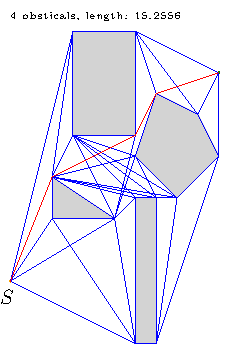
\includegraphics[width=6cm]{figures/correctness1.pdf}
		\caption{}
		\label{fig:correctness_1}
	\end{subfigure}
	\begin{subfigure}{.5\textwidth}
		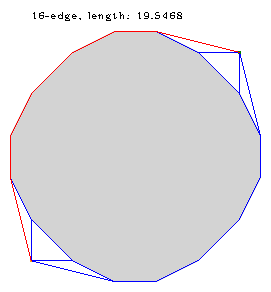
\includegraphics[width=6cm]{figures/correctness2.pdf}
		\caption{}
		\label{fig:correctness_2}
	\end{subfigure}
	\caption{Examples of figures for correctness}
\end{figure}

\subsection{Running time of algorithm}
To test the running time of our implementation we auto generated a map consisting of
x times x squares and put $s$ and $t$ in opposite corners of the map (see figure
\ref{fig:test})

\begin{figure}[H]
    \centering
	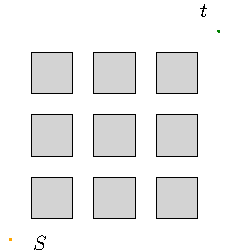
\includegraphics[width=6cm]{figures/testexample.pdf}
	\caption{Examples of figures for correctness}
	\label{fig:test}
\end{figure}
\label{testfilegeneration}
We ran the implementation with the number of violations being constant at $5$ and the
number of vertices was $n= 4 \cdot t^2$ for $t=1,\dots,41$ and got the following graph

\begin{center}
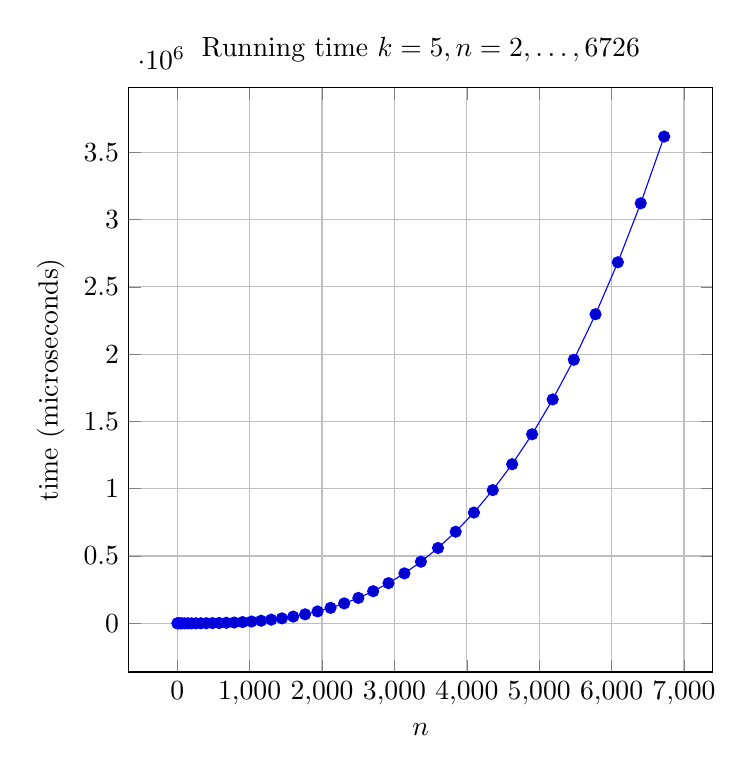
\begin{tikzpicture}
\begin{axis}[
		%xmode=log,
title={Running time $k=5,n=2,\dots,6726$},
height=9cm,
width=9cm,
grid=major,
xlabel = $n$,
ylabel = time (microseconds),
]
\addplot coordinates {
	(2,0)
	(6,0)
	(18,0)
	(38,1)
	(66,9)
	(102,24)
	(146,50)
	(198,112)
	(258,235)
	(326,466)
	(402,848)
	(486,1481)
	(578,2462)
	(678,3939)
	(786,6083)
	(902,9271)
	(1026,13357)
	(1158,19278)
	(1298,27520)
	(1446,37018)
	(1602,50129)
	(1766,66930)
	(1938,88378)
	(2118,114971)
	(2306,148055)
	(2502,188859)
	(2706,238534)
	(2918,298675)
	(3138,371052)
	(3366,457771)
	(3602,559747)
	(3846,680632)
	(4098,822848)
	(4358,989762)
	(4626,1182116)
	(4902,1404667)
	(5186,1663503)
	(5478,1958169)
	(5778,2296425)
	(6086,2682430)
	(6402,3120744)
	(6726,3616376)
};
\end{axis}
\end{tikzpicture}

\end{center}

Then we tried figuring out where the time was spent so we tried measuring the
crossing function, the construction of visibility graph and the Dijkstra
separately and got the following

\begin{center}
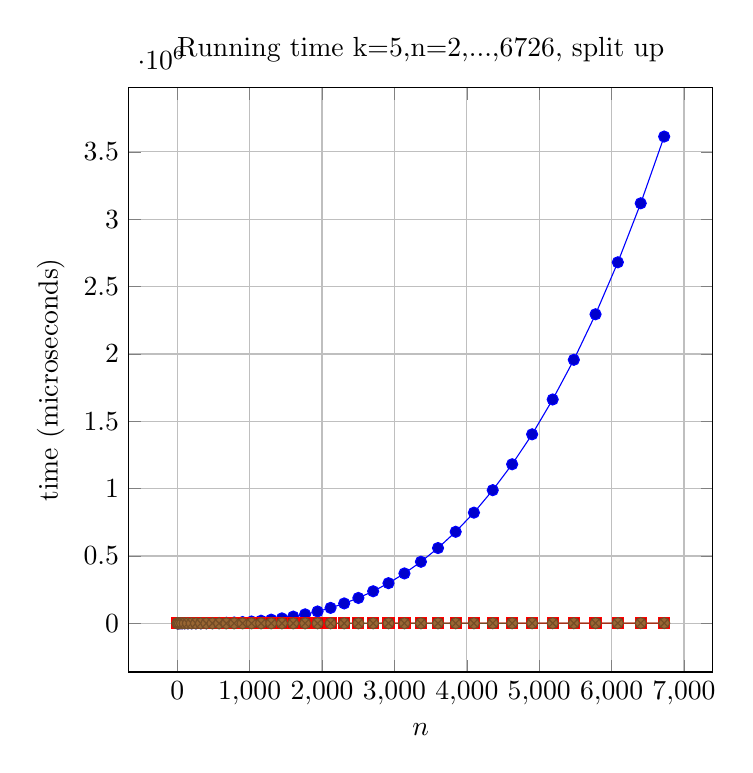
\begin{tikzpicture}
\begin{axis}[
title={Running time k=5,n=2,...,6726, split up},
height=9cm,
width=9cm,
grid=major,
xlabel = $n$,
ylabel = time (microseconds),
]
\addplot coordinates {
%crossing
	(2,0)
	(6,0)
	(18,0)
	(38,1)
	(66,8)
	(102,22)
	(146,45)
	(198,104)
	(258,222)
	(326,447)
	(402,821)
	(486,1444)
	(578,2415)
	(678,3878)
	(786,6006)
	(902,9178)
	(1026,13244)
	(1158,19144)
	(1298,27359)
	(1446,36821)
	(1602,49895)
	(1766,66658)
	(1938,88071)
	(2118,114616)
	(2306,147650)
	(2502,188395)
	(2706,237995)
	(2918,298074)
	(3138,370383)
	(3366,457025)
	(3602,558914)
	(3846,679704)
	(4098,821822)
	(4358,988634)
	(4626,1180886)
	(4902,1403311)
	(5186,1662007)
	(5478,1956547)
	(5778,2294661)
	(6086,2680522)
	(6402,3118674)
	(6726,3614138)
};
\addplot coordinates {
%visibility 
	(2,0)
	(6,0)
	(18,0)
	(38,0)
	(66,0)
	(102,0)
(146,1)
(198,2)
(258,3)
(326,4)
(402,6)
(486,9)
(578,11)
(678,15)
(786,18)
(902,22)
(1026,28)
(1158,33)
(1298,40)
(1446,47)
(1602,56)
(1766,65)
(1938,75)
(2118,87)
(2306,100)
(2502,115)
(2706,131)
(2918,148)
(3138,167)
(3366,190)
(3602,213)
(3846,238)
(4098,264)
(4358,298)
(4626,328)
(4902,363)
(5186,400)
(5478,440)
(5778,481)
(6086,530)
(6402,574)
(6726,628)
};
\addplot coordinates {
%Dijkstra
	(2,0)
(6,0)
(18,0)
(38,0)
(66,1)
(102,2)
(146,4)
(198,6)
(258,10)
(326,15)
(402,21)
(486,28)
(578,36)
(678,46)
(786,59)
(902,71)
(1026,85)
(1158,101)
(1298,121)
(1446,150)
(1602,178)
(1766,207)
(1938,232)
(2118,268)
(2306,305)
(2502,349)
(2706,408)
(2918,453)
(3138,502)
(3366,556)
(3602,620)
(3846,690)
(4098,762)
(4358,830)
(4626,902)
(4902,993)
(5186,1096)
(5478,1182)
(5778,1283)
(6086,1378)
(6402,1496)
(6726,1610)
};
\end{axis}
\end{tikzpicture}

\end{center}

The implementation is totally dominated by the crossing calculating which makes
sense since the $O(n^3)$ is the most dominant sub time, we tried dividing the first graph
with $O(n^3)$ and got the following

\begin{center}
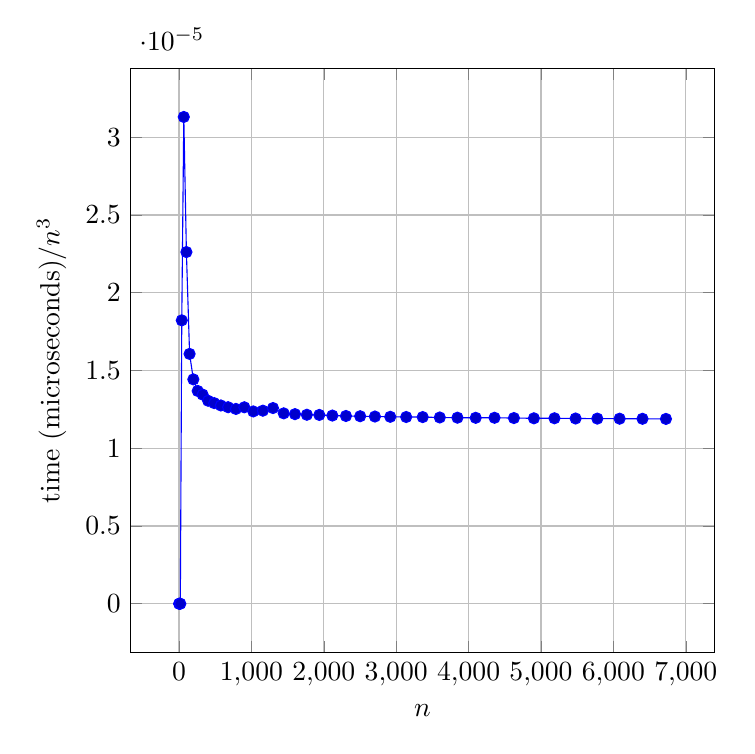
\begin{tikzpicture}
\begin{axis}[
height=9cm,
width=9cm,
grid=major,
xlabel = $n$,
ylabel = time (microseconds)/$n^3$,
]
\addplot coordinates {
	(2,0)
	(6,0)
	(18,0)
	(38,1.82242309374544E-05)
	(66,3.13047833708991E-05)
	(102,2.26157360291291E-05)
	(146,1.60661359272217E-05)
	(198,1.44285421297971E-05)
	(258,1.36838638480003E-05)
	(326,1.34503354733029E-05)
	(402,1.3053221060855E-05)
	(486,1.29016795495295E-05)
	(578,1.27498340864401E-05)
	(678,1.26385397648696E-05)
	(786,1.25270894447943E-05)
	(902,1.26330137388433E-05)
	(1026,1.2367070702209E-05)
	(1158,1.24147019560424E-05)
	(1298,1.25841634982224E-05)
	(1446,1.2243570102851E-05)
	(1602,1.21927454179994E-05)
	(1766,1.2152027041557E-05)
	(1938,1.21417937429069E-05)
	(2118,1.21006985351175E-05)
	(2306,1.20738331437455E-05)
	(2502,1.20580136097767E-05)
	(2706,1.20383485707373E-05)
	(2918,1.20210667777948E-05)
	(3138,1.20081459851104E-05)
	(3366,1.20034459584254E-05)
	(3602,1.19773474781993E-05)
	(3846,1.19642236814143E-05)
	(4098,1.19564913967957E-05)
	(4358,1.19582904652676E-05)
	(4626,1.19410690659842E-05)
	(4902,1.19248646628465E-05)
	(5186,1.19268580687987E-05)
	(5478,1.19119836093996E-05)
	(5778,1.19047328401354E-05)
	(6086,1.1899605218836E-05)
	(6402,1.18935399250374E-05)
	(6726,1.18851040850164E-05)
};
\end{axis}
\end{tikzpicture}

\end{center}

Lastly we tried to make a test where $n=25^2$ and $k=1,\dots,25$ and getting
the almost linear graph

\begin{center}
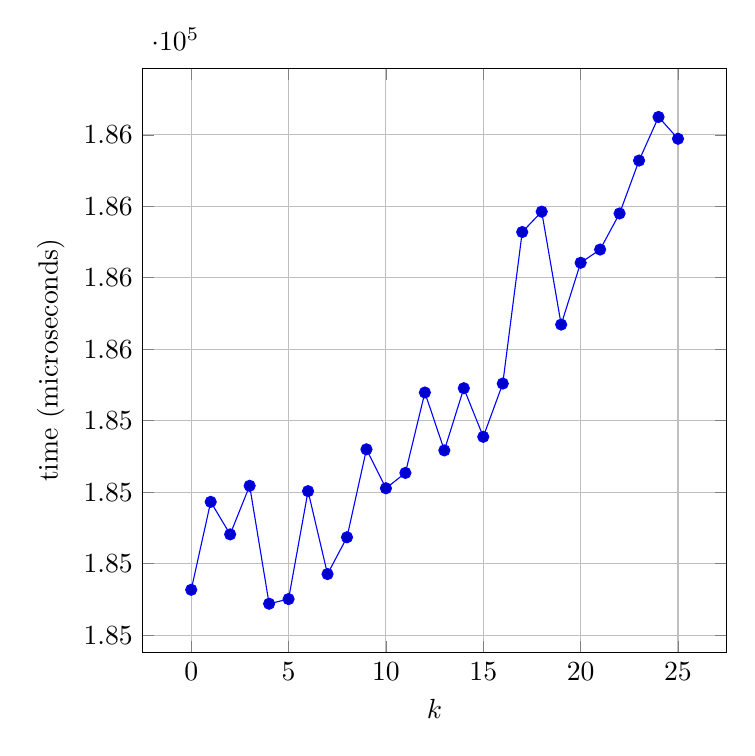
\begin{tikzpicture}
\begin{axis}[
height=9cm,
width=9cm,
grid=major,
xlabel = $k$,
ylabel = time (microseconds),
]

\addplot coordinates {
	(0,184927)
	(1,185173)
	(2,185082)
	(3,185218)
	(4,184888)
	(5,184901)
	(6,185203)
	(7,184971)
	(8,185074)
	(9,185320)
	(10,185211)
	(11,185254)
	(12,185479)
	(13,185317)
	(14,185491)
	(15,185355)
	(16,185504)
	(17,185928)
	(18,185985)
	(19,185669)
	(20,185842)
	(21,185879)
	(22,185980)
	(23,186128)
	(24,186250)
	(25,186189)
};
\end{axis}
\end{tikzpicture}

\end{center}

In conclusion we have implemented a naive $O(n^3)$ algorithm and made tests both
for confirming its correctness and its running time of the algorithm.
